%%
% Copyright (c) 2017 - 2025, Pascal Wagler;
% Copyright (c) 2014 - 2025, John MacFarlane
%
% All rights reserved.
%
% Redistribution and use in source and binary forms, with or without
% modification, are permitted provided that the following conditions
% are met:
%
% - Redistributions of source code must retain the above copyright
% notice, this list of conditions and the following disclaimer.
%
% - Redistributions in binary form must reproduce the above copyright
% notice, this list of conditions and the following disclaimer in the
% documentation and/or other materials provided with the distribution.
%
% - Neither the name of John MacFarlane nor the names of other
% contributors may be used to endorse or promote products derived
% from this software without specific prior written permission.
%
% THIS SOFTWARE IS PROVIDED BY THE COPYRIGHT HOLDERS AND CONTRIBUTORS
% "AS IS" AND ANY EXPRESS OR IMPLIED WARRANTIES, INCLUDING, BUT NOT
% LIMITED TO, THE IMPLIED WARRANTIES OF MERCHANTABILITY AND FITNESS
% FOR A PARTICULAR PURPOSE ARE DISCLAIMED. IN NO EVENT SHALL THE
% COPYRIGHT OWNER OR CONTRIBUTORS BE LIABLE FOR ANY DIRECT, INDIRECT,
% INCIDENTAL, SPECIAL, EXEMPLARY, OR CONSEQUENTIAL DAMAGES (INCLUDING,
% BUT NOT LIMITED TO, PROCUREMENT OF SUBSTITUTE GOODS OR SERVICES;
% LOSS OF USE, DATA, OR PROFITS; OR BUSINESS INTERRUPTION) HOWEVER
% CAUSED AND ON ANY THEORY OF LIABILITY, WHETHER IN CONTRACT, STRICT
% LIABILITY, OR TORT (INCLUDING NEGLIGENCE OR OTHERWISE) ARISING IN
% ANY WAY OUT OF THE USE OF THIS SOFTWARE, EVEN IF ADVISED OF THE
% POSSIBILITY OF SUCH DAMAGE.
%%

%%
% This is the Eisvogel pandoc LaTeX template.
%
% For usage information and examples visit the official GitHub page:
% https://github.com/Wandmalfarbe/pandoc-latex-template
%%
% Options for packages loaded elsewhere
\PassOptionsToPackage{unicode}{hyperref}
\PassOptionsToPackage{hyphens}{url}
\PassOptionsToPackage{dvipsnames,svgnames,x11names,table}{xcolor}
\documentclass[
  american,
  11pt,
  letterpaper,
  oneside  ,captions=tableheading
]{scrartcl}
\usepackage{xcolor}
\usepackage[margin=1in]{geometry}
\usepackage{amsmath,amssymb}

% add backlinks to footnote references, cf. https://tex.stackexchange.com/questions/302266/make-footnote-clickable-both-ways
\usepackage{footnotebackref}
\setcounter{secnumdepth}{5}
\usepackage{iftex}
\ifPDFTeX
  \usepackage[T1]{fontenc}
  \usepackage[utf8]{inputenc}
  \usepackage{textcomp} % provide euro and other symbols
\else % if luatex or xetex
  \usepackage{unicode-math} % this also loads fontspec
  \defaultfontfeatures{Scale=MatchLowercase}
  \defaultfontfeatures[\rmfamily]{Ligatures=TeX,Scale=1}
\fi
\usepackage{lmodern}
\ifPDFTeX\else
  % xetex/luatex font selection
  \setmainfont[]{DejaVu Serif}
  \setsansfont[]{DejaVu Sans}
  \setmonofont[]{DejaVu Sans Mono}
\fi
% Use upquote if available, for straight quotes in verbatim environments
\IfFileExists{upquote.sty}{\usepackage{upquote}}{}
\IfFileExists{microtype.sty}{% use microtype if available
  \usepackage[]{microtype}
  \UseMicrotypeSet[protrusion]{basicmath} % disable protrusion for tt fonts
}{}

\usepackage{setspace}
\makeatletter
\@ifundefined{KOMAClassName}{% if non-KOMA class
  \IfFileExists{parskip.sty}{%
    \usepackage{parskip}
  }{% else
    \setlength{\parindent}{0pt}
    \setlength{\parskip}{6pt plus 2pt minus 1pt}}
}{% if KOMA class
  \KOMAoptions{parskip=half}}
\makeatother
\usepackage{listings}
\newcommand{\passthrough}[1]{#1}
\lstset{defaultdialect=[5.3]Lua}
\lstset{defaultdialect=[x86masm]Assembler}
\usepackage{etoolbox}
\BeforeBeginEnvironment{lstlisting}{\par\noindent\begin{minipage}{\linewidth}}
\AfterEndEnvironment{lstlisting}{\end{minipage}\par\addvspace{\topskip}}
\usepackage{longtable,booktabs,array}
\newcounter{none} % for unnumbered tables
\usepackage{calc} % for calculating minipage widths
% Correct order of tables after \paragraph or \subparagraph
\usepackage{etoolbox}
\makeatletter
\patchcmd\longtable{\par}{\if@noskipsec\mbox{}\fi\par}{}{}
\makeatother
% Allow footnotes in longtable head/foot
\IfFileExists{footnotehyper.sty}{\usepackage{footnotehyper}}{\usepackage{footnote}}
\makesavenoteenv{longtable}
% definitions for citeproc citations
\NewDocumentCommand\citeproctext{}{}
\NewDocumentCommand\citeproc{mm}{%
  \begingroup\def\citeproctext{#2}\cite{#1}\endgroup}
\makeatletter
 % allow citations to break across lines
 \let\@cite@ofmt\@firstofone
 % avoid brackets around text for \cite:
 \def\@biblabel#1{}
 \def\@cite#1#2{{#1\if@tempswa , #2\fi}}
\makeatother
\newlength{\cslhangindent}
\setlength{\cslhangindent}{1.5em}
\newlength{\csllabelwidth}
\setlength{\csllabelwidth}{3em}
\newenvironment{CSLReferences}[2] % #1 hanging-indent, #2 entry-spacing
 {\begin{list}{}{%
  \setlength{\itemindent}{0pt}
  \setlength{\leftmargin}{0pt}
  \setlength{\parsep}{0pt}
  % turn on hanging indent if param 1 is 1
  \ifodd #1
   \setlength{\leftmargin}{\cslhangindent}
   \setlength{\itemindent}{-1\cslhangindent}
  \fi
  % set entry spacing
  \setlength{\itemsep}{#2\baselineskip}}}
 {\end{list}}
\usepackage{calc}
\newcommand{\CSLBlock}[1]{\hfill\break\parbox[t]{\linewidth}{\strut\ignorespaces#1\strut}}
\newcommand{\CSLLeftMargin}[1]{\parbox[t]{\csllabelwidth}{\strut#1\strut}}
\newcommand{\CSLRightInline}[1]{\parbox[t]{\linewidth - \csllabelwidth}{\strut#1\strut}}
\newcommand{\CSLIndent}[1]{\hspace{\cslhangindent}#1}
\ifLuaTeX
\usepackage[bidi=basic,shorthands=off]{babel}
\else
\usepackage[bidi=default,shorthands=off]{babel}
\fi
\ifPDFTeX
\else
\babelfont{rm}[]{DejaVu Serif}
\fi
\ifLuaTeX
  \usepackage{selnolig} % disable illegal ligatures
\fi
\setlength{\emergencystretch}{3em} % prevent overfull lines
\providecommand{\tightlist}{%
  \setlength{\itemsep}{0pt}\setlength{\parskip}{0pt}}
\usepackage{graphicx}
\usepackage{xurl}
\usepackage{rotating}
\usepackage{booktabs}
\usepackage{bookmark}
\IfFileExists{xurl.sty}{\usepackage{xurl}}{} % add URL line breaks if available
\urlstyle{same}
\definecolor{default-linkcolor}{HTML}{A50000}
\definecolor{default-filecolor}{HTML}{A50000}
\definecolor{default-citecolor}{HTML}{4077C0}
\definecolor{default-urlcolor}{HTML}{4077C0}

\hypersetup{
  pdftitle={Healthcare Analytics Challenges: A Three-Pillar Framework Connecting Analytics Maturity, Workforce Agility, and Technical Enablement},
  pdfauthor={Samuel T Harrold, Yuimedi},
  pdflang={en-US},
  pdfkeywords={healthcare analytics, healthcare informatics, analytical
framework, analytics maturity, workforce turnover, institutional
memory, text-to-SQL, natural language processing, knowledge
portal, conversational AI},
  colorlinks=true,
  linkcolor={blue},
  filecolor={default-filecolor},
  citecolor={blue},
  urlcolor={blue},
  breaklinks=true,
  pdfcreator={LaTeX via pandoc with the Eisvogel template}}

\title{Healthcare Analytics Challenges: A Three-Pillar Framework
Connecting Analytics Maturity, Workforce Agility, and Technical
Enablement}
\author{Samuel T Harrold, Yuimedi}
\date{January 2026}


%
% for the background color of the title page
%
\usepackage{pagecolor}
\usepackage{afterpage}

%
% break urls
%
\PassOptionsToPackage{hyphens}{url}

%
% When using babel or polyglossia with biblatex, loading csquotes is recommended
% to ensure that quoted texts are typeset according to the rules of your main language.
%
\usepackage{csquotes}

%
% captions
%
\definecolor{caption-color}{HTML}{777777}
\usepackage[font={stretch=1.2}, textfont={color=caption-color}, position=top, skip=4mm, labelfont=bf, singlelinecheck=false, justification=raggedright]{caption}
\setcapindent{0em}

%
% blockquote
%
\definecolor{blockquote-border}{RGB}{221,221,221}
\definecolor{blockquote-text}{RGB}{119,119,119}
\usepackage{mdframed}
\newmdenv[rightline=false,bottomline=false,topline=false,linewidth=3pt,linecolor=blockquote-border,skipabove=\parskip]{customblockquote}
\renewenvironment{quote}{\begin{customblockquote}\list{}{\rightmargin=0em\leftmargin=0em}%
\item\relax\color{blockquote-text}\ignorespaces}{\unskip\unskip\endlist\end{customblockquote}}

%
% Source Sans Pro as the default font family
% Source Code Pro for monospace text
%
% 'default' option sets the default
% font family to Source Sans Pro, not \sfdefault.
%
% Note that the font has been officially renamed to `Source Sans 3`, and
% the version provided by the `sourcesanspro` package is slightly outdated.
% You can install the newer version locally and use it, for example, with
% `mainfont: "Source Sans 3"` in the YAML metadata (requires XeTeX or LuaTeX).
%
\ifnum 0\ifxetex 1\fi\ifluatex 1\fi=0 % if pdftex
    \usepackage[default]{sourcesanspro}
  \usepackage{sourcecodepro}
  \else % if not pdftex
    \fi

%
% heading color
%
\definecolor{heading-color}{RGB}{40,40,40}
% By default, the KOMA-Script classes will typeset sectioning headings in
% sans-serif. Use the normal body font for headings.
\addtokomafont{disposition}{\normalfont\color{heading-color}\bfseries}

%
% variables for title, author and date
%
\usepackage{titling}
\title{Healthcare Analytics Challenges: A Three-Pillar Framework
Connecting Analytics Maturity, Workforce Agility, and Technical
Enablement}
\author{Samuel T Harrold, Yuimedi}
\date{January 2026}

%
% tables
%

\definecolor{table-row-color}{HTML}{F5F5F5}
\definecolor{table-rule-color}{HTML}{999999}

%\arrayrulecolor{black!40}
\arrayrulecolor{table-rule-color}     % color of \toprule, \midrule, \bottomrule
\setlength\heavyrulewidth{0.3ex}      % thickness of \toprule, \bottomrule
\renewcommand{\arraystretch}{1.3}     % spacing (padding)


%
% remove paragraph indentation
%
\setlength{\parindent}{0pt}
\setlength{\parskip}{6pt plus 2pt minus 1pt}
\setlength{\emergencystretch}{3em}  % prevent overfull lines

%
%
% Listings
%
%


%
% general listing colors
%
\definecolor{listing-background}{HTML}{F7F7F7}
\definecolor{listing-rule}{HTML}{B3B2B3}
\definecolor{listing-numbers}{HTML}{B3B2B3}
\definecolor{listing-text-color}{HTML}{000000}
\definecolor{listing-keyword}{HTML}{435489}
\definecolor{listing-keyword-2}{HTML}{1284CA} % additional keywords
\definecolor{listing-keyword-3}{HTML}{9137CB} % additional keywords
\definecolor{listing-identifier}{HTML}{435489}
\definecolor{listing-string}{HTML}{00999A}
\definecolor{listing-comment}{HTML}{8E8E8E}

\lstdefinestyle{eisvogel_listing_style}{
  language         = java,
  numbers          = left,
  xleftmargin      = 2.7em,
  framexleftmargin = 2.5em,
  backgroundcolor  = \color{listing-background},
  basicstyle       = \color{listing-text-color}\linespread{1.0}%
                      \lst@ifdisplaystyle%
                      \small%
                      \fi\ttfamily{},
  breaklines       = true,
  frame            = single,
  framesep         = 0.19em,
  rulecolor        = \color{listing-rule},
  frameround       = ffff,
  tabsize          = 4,
  numberstyle      = \color{listing-numbers},
  aboveskip        = 1.0em,
  belowskip        = 0.1em,
  abovecaptionskip = 0em,
  belowcaptionskip = 1.0em,
  keywordstyle     = {\color{listing-keyword}\bfseries},
  keywordstyle     = {[2]\color{listing-keyword-2}\bfseries},
  keywordstyle     = {[3]\color{listing-keyword-3}\bfseries\itshape},
  sensitive        = true,
  identifierstyle  = \color{listing-identifier},
  commentstyle     = \color{listing-comment},
  stringstyle      = \color{listing-string},
  showstringspaces = false,
  escapeinside     = {/*@}{@*/}, % Allow LaTeX inside these special comments
  literate         =
  {á}{{\'a}}1 {é}{{\'e}}1 {í}{{\'i}}1 {ó}{{\'o}}1 {ú}{{\'u}}1
  {Á}{{\'A}}1 {É}{{\'E}}1 {Í}{{\'I}}1 {Ó}{{\'O}}1 {Ú}{{\'U}}1
  {à}{{\`a}}1 {è}{{\`e}}1 {ì}{{\`i}}1 {ò}{{\`o}}1 {ù}{{\`u}}1
  {À}{{\`A}}1 {È}{{\`E}}1 {Ì}{{\`I}}1 {Ò}{{\`O}}1 {Ù}{{\`U}}1
  {ä}{{\"a}}1 {ë}{{\"e}}1 {ï}{{\"i}}1 {ö}{{\"o}}1 {ü}{{\"u}}1
  {Ä}{{\"A}}1 {Ë}{{\"E}}1 {Ï}{{\"I}}1 {Ö}{{\"O}}1 {Ü}{{\"U}}1
  {â}{{\^a}}1 {ê}{{\^e}}1 {î}{{\^i}}1 {ô}{{\^o}}1 {û}{{\^u}}1
  {Â}{{\^A}}1 {Ê}{{\^E}}1 {Î}{{\^I}}1 {Ô}{{\^O}}1 {Û}{{\^U}}1
  {œ}{{\oe}}1 {Œ}{{\OE}}1 {æ}{{\ae}}1 {Æ}{{\AE}}1 {ß}{{\ss}}1
  {ç}{{\c c}}1 {Ç}{{\c C}}1 {ø}{{\o}}1 {å}{{\r a}}1 {Å}{{\r A}}1
  {€}{{\EUR}}1 {£}{{\pounds}}1 {«}{{\guillemotleft}}1
  {»}{{\guillemotright}}1 {ñ}{{\~n}}1 {Ñ}{{\~N}}1 {¿}{{?`}}1
  {…}{{\ldots}}1 {≥}{{>=}}1 {≤}{{<=}}1 {„}{{\glqq}}1 {“}{{\grqq}}1
  {”}{{''}}1
}
\lstset{style=eisvogel_listing_style}

%
% Java (Java SE 12, 2019-06-22)
%
\lstdefinelanguage{Java}{
  morekeywords={
    % normal keywords (without data types)
    abstract,assert,break,case,catch,class,continue,default,
    do,else,enum,exports,extends,final,finally,for,if,implements,
    import,instanceof,interface,module,native,new,package,private,
    protected,public,requires,return,static,strictfp,super,switch,
    synchronized,this,throw,throws,transient,try,volatile,while,
    % var is an identifier
    var
  },
  morekeywords={[2] % data types
    % primitive data types
    boolean,byte,char,double,float,int,long,short,
    % String
    String,
    % primitive wrapper types
    Boolean,Byte,Character,Double,Float,Integer,Long,Short
    % number types
    Number,AtomicInteger,AtomicLong,BigDecimal,BigInteger,DoubleAccumulator,DoubleAdder,LongAccumulator,LongAdder,Short,
    % other
    Object,Void,void
  },
  morekeywords={[3] % literals
    % reserved words for literal values
    null,true,false,
  },
  sensitive,
  morecomment  = [l]//,
  morecomment  = [s]{/*}{*/},
  morecomment  = [s]{/**}{*/},
  morestring   = [b]",
  morestring   = [b]',
}

\lstdefinelanguage{XML}{
  morestring      = [b]",
  moredelim       = [s][\bfseries\color{listing-keyword}]{<}{\ },
  moredelim       = [s][\bfseries\color{listing-keyword}]{</}{>},
  moredelim       = [l][\bfseries\color{listing-keyword}]{/>},
  moredelim       = [l][\bfseries\color{listing-keyword}]{>},
  morecomment     = [s]{<?}{?>},
  morecomment     = [s]{<!--}{-->},
  commentstyle    = \color{listing-comment},
  stringstyle     = \color{listing-string},
  identifierstyle = \color{listing-identifier}
}

%
% header and footer
%
\usepackage[headsepline,footsepline]{scrlayer-scrpage}

\newpairofpagestyles{eisvogel-header-footer}{
  \clearpairofpagestyles
  \ihead*{Healthcare Analytics Challenges}
  \chead*{}
  \ohead*{January 2026}
  \ifoot*{\hspace{0pt}}
  \cfoot*{\thepage}
  \ofoot*{\hspace{0pt}}
  \addtokomafont{pageheadfoot}{\upshape}
}
\pagestyle{eisvogel-header-footer}



%
% Define watermark
%

\begin{document}

\begin{titlepage}
\newgeometry{left=6cm}
\definecolor{titlepage-color}{HTML}{FFFFFF}
\newpagecolor{titlepage-color}\afterpage{\restorepagecolor}
\newcommand{\colorRule}[3][black]{\textcolor[HTML]{#1}{\rule{#2}{#3}}}
\begin{flushleft}
\noindent
\\[-1em]
\color[HTML]{000000}
\makebox[0pt][l]{\colorRule[000000]{1.3\textwidth}{2pt}}
\par
\noindent

{
  \setstretch{1.4}
  \vfill
  \noindent {\huge \textbf{\textsf{Healthcare Analytics Challenges: A
Three-Pillar Framework Connecting Analytics Maturity, Workforce Agility,
and Technical Enablement}}}
    \vskip 2em
  \noindent {\Large \textsf{Samuel T Harrold, Yuimedi}}
  \vfill
}


\textsf{January 2026}
\end{flushleft}
\end{titlepage}
\restoregeometry
\pagenumbering{arabic}

% don't generate the default title
% \maketitle
\begin{abstract}
\textbf{Background:} Healthcare organizations face three interconnected
challenges: low analytics maturity, with only 39 organizations globally
having achieved HIMSS AMAM Stage 6-7; systemic instability from high
leadership turnover (53\% of CIOs with \textless3 years tenure) and
persistent digital skills shortages; and technical barriers in natural
language to SQL generation. When these challenges interact, they create
institutional memory loss that threatens data-driven healthcare
transformation.

\textbf{Objective:} This research develops a three-pillar analytical
framework connecting analytics maturity, workforce agility, and
technical enablement. The framework reveals how these capabilities
interconnect and compound each other.

\textbf{Methods:} We conducted a narrative literature review of
peer-reviewed studies and industry reports on natural language to SQL
(NL2SQL) generation, healthcare analytics maturity, and workforce
turnover. Grey literature was assessed using the AACODS checklist.
Evidence was synthesized through the three-pillar analytical framework
to examine how these challenges interconnect and compound.

\textbf{Results:} Healthcare-specific text-to-SQL benchmarks show
significant progress, though current models are ``not yet sufficiently
accurate for unsupervised use'' in clinical settings. Most healthcare
organizations remain at HIMSS AMAM Stages 0-3 with limited predictive
capabilities. Healthcare IT turnover significantly exceeds other IT
sectors, creating measurable institutional memory loss. The framework
reveals a compounding dynamic: low-maturity organizations experience
higher turnover, which degrades the institutional knowledge needed for
maturity advancement, while technical barriers prevent the capture of
expertise before it is lost.

\textbf{Conclusions:} We contribute a three-pillar analytical framework
synthesizing evidence on analytics maturity, workforce agility, and
technical enablement. The framework reveals a compounding effect: low
maturity accelerates turnover, which degrades maturity, and low
enablement prevents recovery. This analytical lens enables
organizational self-assessment and informs future research on
technological interventions, such as conversational AI platforms.
\end{abstract}


{
\setcounter{tocdepth}{3}
\tableofcontents
}
\setstretch{1.15}
\section{Introduction}\label{introduction}

\subsection{The Compounding Crisis in Healthcare
Analytics}\label{the-compounding-crisis-in-healthcare-analytics}

Healthcare organizations face three critical, interconnected challenges
that form a compounding crisis, collectively threatening their ability
to become data-driven enterprises. Unlike technology or financial
services, healthcare combines complex clinical workflows, extensive
regulatory requirements, and a workforce with limited technical training
but deep domain expertise (\citeproc{ref-american2023}{1}). This paper
introduces a three-pillar framework that examines how these challenges
interconnect and reinforce one another.

The framework follows a logical progression from observation to root
cause:

\begin{enumerate}
\def\labelenumi{\arabic{enumi}.}
\item
  \textbf{Pillar 1: Low Analytics Maturity (The Observation):} The most
  visible symptom is healthcare's struggle to advance its analytics
  capabilities. Despite massive investments in data infrastructure, most
  organizations remain at low maturity levels, unable to leverage their
  data for predictive or prescriptive insights.
\item
  \textbf{Pillar 2: Workforce Instability (The Cause):} This low
  maturity is not a static state but is actively driven by a systemic
  workforce crisis. High turnover at leadership, operational, and
  specialized levels creates a constant drain of institutional
  knowledge, preventing the accumulation of expertise required for
  maturity advancement.
\item
  \textbf{Pillar 3: Technical Barriers (The Root Mechanism):} The cycle
  is perpetuated by technical barriers that prevent organizations from
  capturing expertise before it is lost. The gap between clinical domain
  experts and the technical skills required for data access (e.g., SQL)
  creates a dependency on a small pool of specialists, making the system
  fragile and vulnerable to knowledge loss.
\end{enumerate}

This introduction will now examine the evidence for each of these
pillars in turn, establishing the foundation for the integrated
framework that is the central contribution of this paper.

\subsection{Pillar 1: Low Healthcare Analytics
Maturity}\label{pillar-1-low-healthcare-analytics-maturity}

The Healthcare Information Management Systems Society (HIMSS) Analytics
Maturity Assessment Model (AMAM) provides the industry standard for
measuring analytics capabilities. Recent assessments reveal a sobering
reality: as of late 2024, only 26 organizations worldwide had achieved
Stage 6 maturity, with merely 13 reaching Stage 7
(\citeproc{ref-himss2024}{2},\citeproc{ref-himss2024news}{3}). Despite
this progress, the vast majority of organizations remain at Stages 0-3,
characterized by fragmented data, limited automated reporting, and
minimal predictive capabilities (\citeproc{ref-himss2024}{2}). This low
maturity severely constrains evidence-based decision making.

\subsection{Pillar 2: Institutional Memory Loss from Workforce
Instability}\label{pillar-2-institutional-memory-loss-from-workforce-instability}

Healthcare faces an institutional memory crisis that has evolved from
simple turnover to systemic instability. This crisis unfolds at three
levels:

\begin{itemize}
\tightlist
\item
  \textbf{Strategic Level:} Leadership churn is acute, with 53\% of
  healthcare CIOs having a tenure of less than three years, leading to
  frequent shifts in analytics strategy
  (\citeproc{ref-wittkieffer2024}{4}).
\item
  \textbf{Operational Level:} 79\% of healthcare provider organizations
  report persistent shortages in ``Information and Digital Health''
  roles, leaving critical technical positions vacant
  (\citeproc{ref-himssworkforce2024}{5}).
\item
  \textbf{Foundational Level:} A 2025 analysis found that 55\% of public
  health informatics specialists intended to leave their positions,
  preventing the accumulation of the tacit knowledge needed to maintain
  analytics infrastructure (\citeproc{ref-rajamani2025}{6}).
\end{itemize}

This multi-layered churn creates a cascade of knowledge loss. When
experienced analysts leave, they take with them irreplaceable tacit
knowledge: business rules, data anomalies, and analytical context that
traditional documentation fails to capture. The challenge is not new; a
foundational 2004 study established that healthcare IT staff had the
lowest expected tenure for new hires among all IT sectors at just 2.9
years (\citeproc{ref-ang2004}{7}). That this two-decade-old study
remains a key benchmark is itself evidence of the crisis: the industry
is so unstable it has lost the ability to track its own attrition.

\subsection{Pillar 3: Technical Barriers to Data
Access}\label{pillar-3-technical-barriers-to-data-access}

Against this backdrop of organizational immaturity and workforce
instability, technical barriers perpetuate the cycle. Accessing
healthcare insights requires navigating a complex technical landscape.
While the immediate barrier is often the ``technical skills
gap''---where clinical experts lack SQL expertise---this is merely the
surface of deeper challenges in \textbf{Semantic Interoperability} and
\textbf{Data Quality}
(\citeproc{ref-gal2019}{8},\citeproc{ref-zhang2024}{9}).

In this context, Natural Language to SQL (NL2SQL) generation is not a
``magic bullet'' but a democratizing \textbf{Interface Layer} and a
\textbf{Governance Forcing Function}. For an AI system to translate a
natural language question into a correct SQL query, technical
prerequisites must be met: validated data models, explicit business
logic, and codified definitions. The AI interface forces the
organization to make this knowledge explicit, moving it from the minds
of a few experts into a durable, shared system. It provides a bridge
that allows non-technical domain experts to interact with data
\emph{alongside} these modernization efforts, unlocking value from
imperfect systems while broader interoperability efforts continue
(\citeproc{ref-anthropic2025}{10}--\citeproc{ref-arora2025}{13}).

The implications of these three interconnected challenges are measurable
in both operational and clinical terms. When analytics barriers are
addressed, outcomes improve substantially: one Medicare ACO reduced
readmission rates from 24\% to 17.8\% and achieved \$1.6 million in cost
savings by implementing data analytics to overcome EHR fragmentation
(\citeproc{ref-latrella2024}{14}). Yet, barriers remain pervasive, with
68\% of healthcare organizations citing data interoperability as the
leading obstacle, followed by privacy concerns (64\%) and insufficient
staff training (59\%) (\citeproc{ref-nashid2023}{15}). Adoption of big
data analytics faces validated barriers including employee resistance to
change and lack of organizational readiness, which directly stall
data-driven initiatives
(\citeproc{ref-shahbaz2019}{16},\citeproc{ref-kamble2019}{17}).
Together, these three pillars represent a compounding cycle of
operational inefficiencies with demonstrated implications for healthcare
delivery.

\subsection{Objectives}\label{objectives}

This research aims to develop a framework for understanding healthcare's
interconnected analytics challenges. The specific objectives are as
follows:

\subsubsection{Primary Objective}\label{primary-objective}

Develop and validate a three-pillar analytical framework that explains
how analytics maturity, workforce agility, and technical enablement
interconnect and compound each other.

\subsubsection{Secondary Objectives}\label{secondary-objectives}

\begin{enumerate}
\def\labelenumi{\arabic{enumi}.}
\tightlist
\item
  \textbf{Synthesize current evidence} on natural language to SQL
  generation as a technical barrier.
\item
  \textbf{Document the extent} of analytics maturity challenges in
  healthcare organizations globally.
\item
  \textbf{Quantify the impact} of workforce turnover on institutional
  memory and analytics capabilities.
\item
  \textbf{Reveal interconnections} between the three pillars through
  evidence synthesis.
\item
  \textbf{Provide an assessment rubric} for organizational
  self-evaluation.
\end{enumerate}

\subsubsection{Non-Goals}\label{non-goals}

This research does not address:

\begin{itemize}
\tightlist
\item
  Specific vendor comparisons or product recommendations.
\item
  Implementation details for particular healthcare IT environments.
\item
  Regulatory compliance strategies for specific jurisdictions.
\item
  Technical architecture specifications for conversational AI systems.
\end{itemize}

\emph{Note: Analysis of market dynamics and structural factors
explaining why institution-specific analytics challenges persist is
within the scope of this paper. This market-level analysis provides
context for evaluating solution approaches and differs from product
comparisons, which would evaluate or recommend specific vendor
offerings.}

\subsection{Contributions}\label{contributions}

This paper makes the following contributions to the healthcare
informatics literature:

\begin{enumerate}
\def\labelenumi{\arabic{enumi}.}
\item
  \textbf{Three-Pillar Analytical Framework}: We synthesize evidence
  from three disconnected research domains---healthcare analytics
  maturity, workforce turnover, and natural language processing---into a
  unified analytical framework. This framework reveals how these
  challenges interconnect and compound each other: low maturity
  accelerates turnover, turnover degrades agility, and low technical
  enablement prevents recovery. The framework provides a lens for
  organizational self-assessment and research prioritization.
\item
  \textbf{Evidence Synthesis}: We document the current state of each
  pillar through a comprehensive literature review, providing healthcare
  organizations with consolidated evidence on analytics maturity
  benchmarks, the impact of workforce turnover, and NL2SQL technical
  capabilities.
\item
  \textbf{Illustrative Application}: Drawing on established knowledge
  management literature, we describe the validated query cycle as an
  example of how the framework can inform technology design. This
  concept addresses institutional memory loss through a six-step process
  that allows domain experts to validate and store queries, ensuring
  that knowledge persists independently of staff tenure. Figures 1 and 2
  illustrate this architecture and cycle.
\end{enumerate}

\begin{figure}[htbp]
\centering
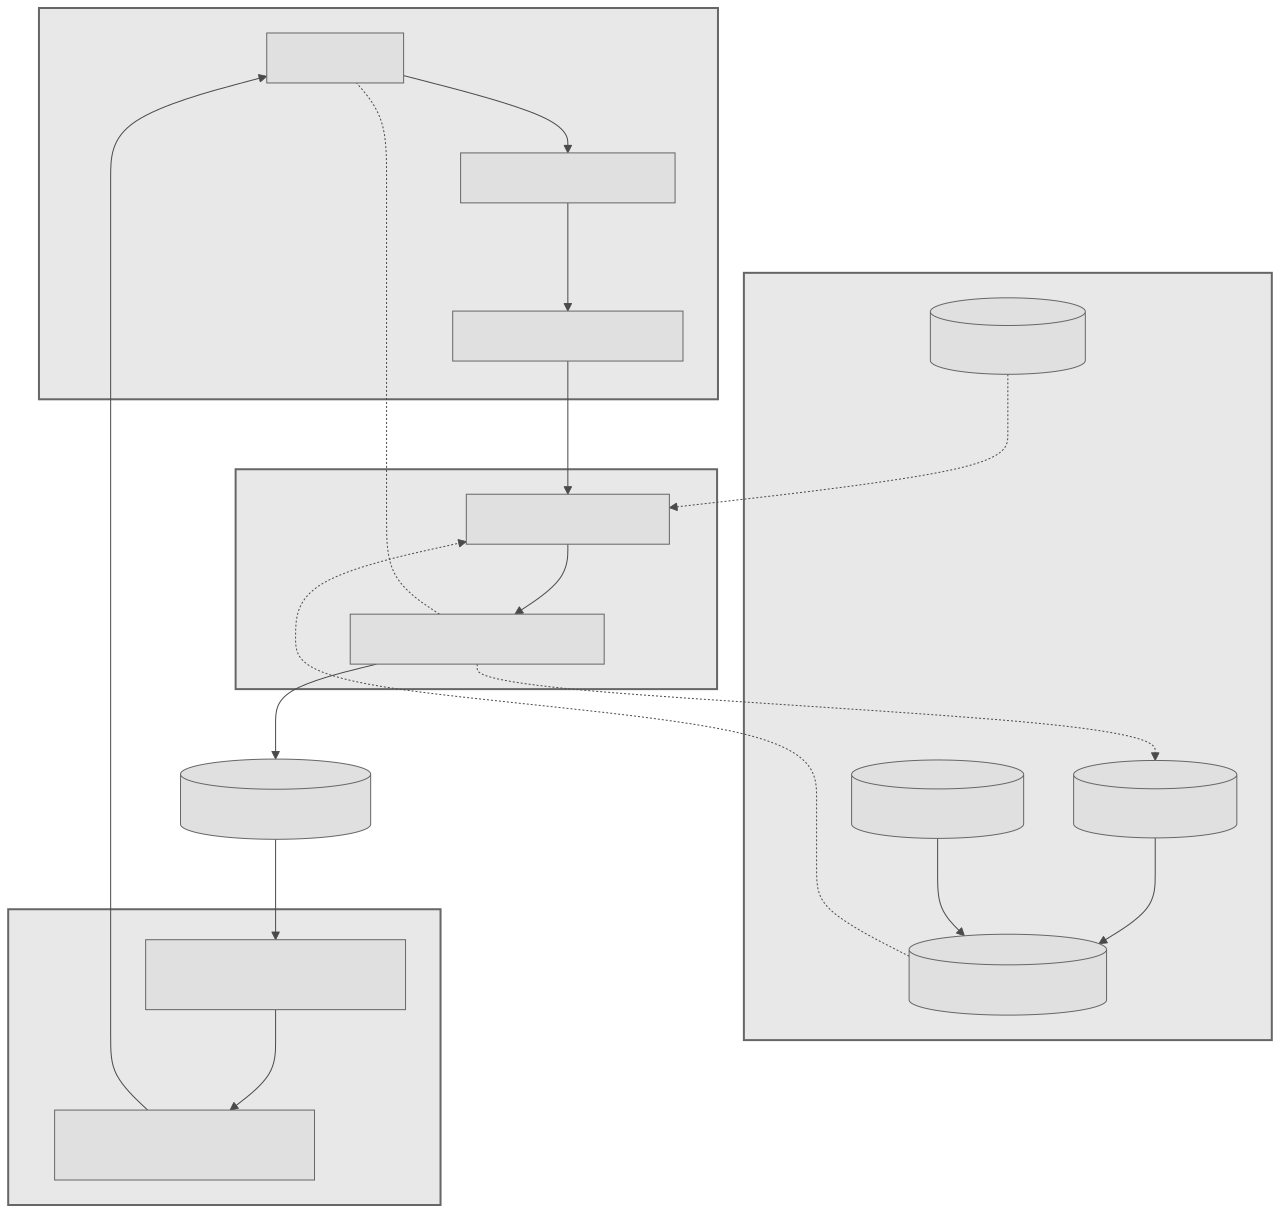
\includegraphics[width=0.95\textwidth,keepaspectratio]{figures/architecture.mmd.png}
\caption{Healthcare Analytics Architecture. Solid lines indicate the primary data flow from clinical user natural language queries through a conversational AI interface to a healthcare NLP engine for context-aware SQL generation. Bi-directional arrows at steps 5 and 8 represent the iterative 'Query \& Refine' loop where users refine their intent based on delivered insights. The critical validation step (dotted bi-directional line) shows domain experts confirming or correcting generated SQL before results are trusted. Validated NL+SQL pairs flow to organizational memory (dashed line), where they persist independent of staff tenure and inform future query generation.}
\label{fig:architecture}
\end{figure}

\subsubsection{Illustrative Application: The Validated Query Cycle as a
Governance Forcing
Function}\label{illustrative-application-the-validated-query-cycle-as-a-governance-forcing-function}

To demonstrate how the three-pillar framework might inform technology
design, we describe a validated query cycle. This cycle functions as a
\textbf{Governance Forcing Function}, a mechanism that uses technical
implementation to compel the adoption of stronger data governance
practices. It directly addresses institutional memory loss (Pillar 2) by
systematically converting tacit knowledge into an explicit, durable
asset, thereby reducing technical barriers (Pillar 3) and enabling
organizations to advance their analytics maturity (Pillar 1).

The six-step cycle (Figure 2) illustrates this approach:

\begin{enumerate}
\def\labelenumi{\arabic{enumi}.}
\item
  \textbf{Query}: A domain expert (clinician, analyst, or administrator)
  asks a natural language question, such as, ``What was our 30-day
  readmission rate for heart failure patients last quarter?''
\item
  \textbf{Generation}: The conversational AI system generates candidate
  SQL code, leveraging healthcare ontologies and organizational schema
  knowledge.
\item
  \textbf{Validation}: The AI provides a natural language explanation of
  the SQL logic and results, allowing the domain expert to validate the
  query's intent without reviewing raw code. This human-in-the-loop step
  aligns with ``Human-on-the-Loop'' (HotL) frameworks, transforming
  validation from a binary check into an iterative knowledge capture
  process
  (\citeproc{ref-bravorocca2023}{18},\citeproc{ref-mosqueirarey2023}{19}).
  This is essential given that current models are ``not yet sufficiently
  accurate for unsupervised use'' in clinical settings
  (\citeproc{ref-ziletti2024}{20}).
\item
  \textbf{Storage}: Once validated, the NL+SQL pair is stored in
  organizational memory as a durable knowledge artifact, along with
  mandatory ``Rationale Metadata'' documenting the query's business
  logic (e.g., ``Excluding Hospice per 2025 CMS rules'').
\item
  \textbf{Retrieval}: When future users ask similar questions, the
  system retrieves relevant validated pairs, reducing dependence on
  individual expertise.
\item
  \textbf{Persistence}: When the original expert leaves, their
  analytical knowledge remains embedded in the system. New staff inherit
  executable knowledge rather than starting from scratch.
\end{enumerate}

\begin{figure}[htbp]
\centering
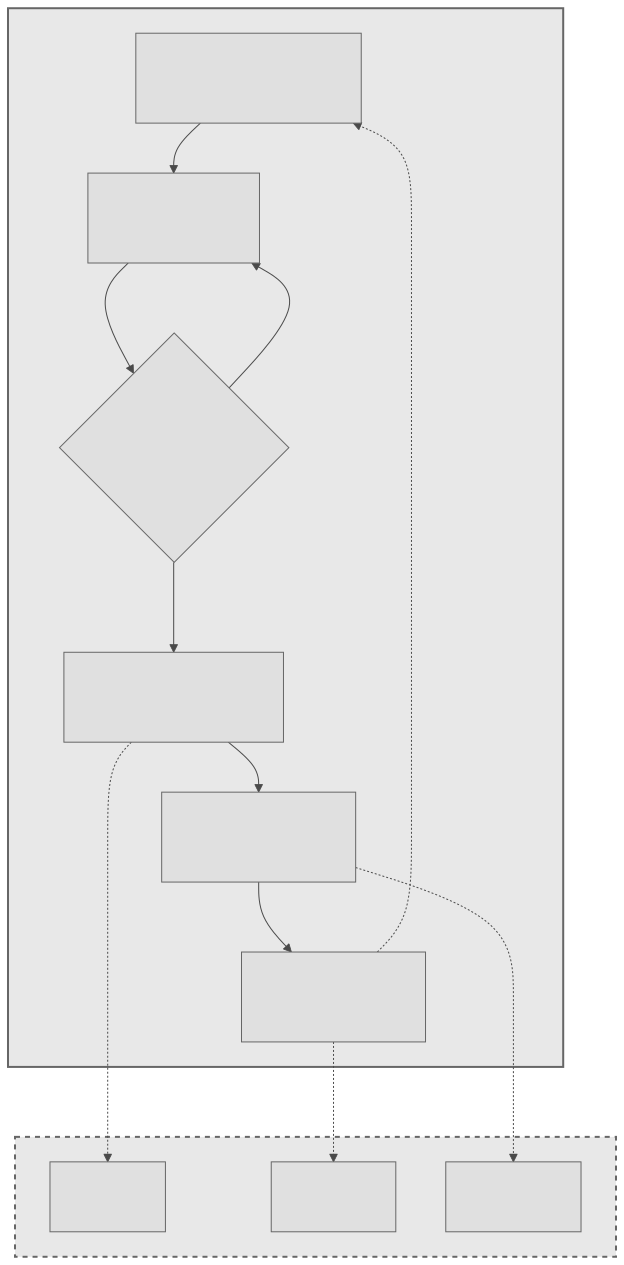
\includegraphics[width=0.5\textwidth,keepaspectratio]{figures/knowledge-cycle.mmd.png}
\caption{The Validated Query Cycle, shown as six numbered steps in the diagram. (1) Domain experts ask natural language questions, (2) the system generates candidate SQL, (3) AI provides a natural language explanation of the SQL logic; domain expert confirms the intent and results, (4) validated pairs are stored, (5) future queries retrieve validated knowledge, and (6) expertise persists through staff turnover. This cycle breaks the compounding effect where turnover erases institutional memory.}
\label{fig:knowledge-cycle}
\end{figure}

This cycle breaks the compounding effect identified in the three-pillar
framework: turnover no longer erases analytical knowledge because
expertise is embedded in validated query pairs rather than individual
memory. Low-maturity organizations can accelerate advancement by
accumulating validated queries, and technical barriers are reduced
because new staff access proven query patterns rather than recreating
analytical logic.

\subsection{Document Structure}\label{document-structure}

Following this introduction, the paper proceeds through five main
sections. The Methodology section describes the narrative review
approach, literature search strategy, and source selection criteria. The
Framework Development section documents how the three-pillar framework
emerged from the literature and its theoretical grounding. The
Literature Review synthesizes evidence across the three pillar domains:
natural language to SQL generation, analytics maturity, and workforce
dynamics. The Discussion examines implications, limitations, and future
research directions. Finally, the Conclusion summarizes the three-pillar
analytical framework as this paper's primary contribution to healthcare
informatics literature.

\section{Methodology}\label{methodology}

\subsection{Review Approach}\label{review-approach}

This paper employs a narrative review methodology to synthesize evidence
across the three pillars of the framework: analytics maturity, workforce
agility, and technical enablement (specifically natural language to SQL
generation). Unlike systematic reviews that follow pre-registered
protocols with exhaustive searches, narrative reviews provide expert
synthesis of relevant literature to construct coherent arguments and
identify patterns across diverse evidence sources.

The narrative review approach was selected because:

\begin{enumerate}
\def\labelenumi{\arabic{enumi}.}
\tightlist
\item
  \textbf{Integration across domains}: The paper synthesizes evidence
  from distinct fields (clinical informatics, human resources, natural
  language processing) that require interpretive integration rather than
  statistical pooling
\item
  \textbf{Original analytical framework}: The three-pillar framework
  emerged iteratively from the literature rather than being
  pre-specified
\item
  \textbf{Heterogeneous evidence types}: The evidence base includes
  peer-reviewed research, industry reports, and benchmark datasets that
  cannot be meaningfully combined through meta-analysis
\end{enumerate}

\subsection{Stage 1: Identification and Targeted
Queries}\label{stage-1-identification-and-targeted-queries}

Literature was identified through multiple channels between January 2023
and December 2025:

\textbf{Academic Databases:}

\begin{itemize}
\tightlist
\item
  Crossref: Cross-disciplinary academic literature, citation metadata
\item
  PubMed: Clinical informatics, healthcare workforce, medical
  administration
\item
  arXiv: Machine learning and NLP preprints, benchmark studies
\item
  Semantic Scholar: AI and computer science papers, citation analysis
\end{itemize}

\textbf{Industry Sources:}

\begin{itemize}
\tightlist
\item
  HIMSS: Analytics Maturity Model documentation and industry standards
\item
  Healthcare providers: NHS Trust implementation case studies
\item
  Market research: Precedence Research, Forrester analyst reports
\item
  Technology vendors: Health Catalyst, Oracle, Anthropic technical
  documentation
\item
  Professional associations: AHIMA/NORC workforce surveys
\item
  Business news: IBM, CNBC coverage of healthcare analytics ventures
\end{itemize}

\textbf{Search Concepts and Results:}

Search terms emerged iteratively and were organized around the
three-pillar framework. Table 1 summarizes the search concepts and
results by source.

\begin{longtable}[]{@{}lccccc@{}}
\caption{Initial search results by database source. Numbers in
parentheses indicate studies passing initial screening. Search concepts:
\textbf{Analytics Maturity} (``healthcare analytics maturity'', ``HIMSS
AMAM'', ``analytics adoption'', ``big data analytics adoption'',
``resistance to change'', ``analytics standardization failure'',
``low-code ROI''); \textbf{Workforce Agility} (``healthcare IT tenure'',
``IT training time'', ``turnover cost'', ``institutional memory loss'',
``organizational forgetting'', ``competence loss'', ``knowledge
portal'', ``SECI model''); \textbf{Technical Enablement} (``NL2SQL
healthcare'', ``text-to-SQL clinical'', ``MIMICSQL'', ``EHRSQL'',
``schema discovery'', ``semantic column matching'', ``vector
embeddings'').}\tabularnewline
\toprule\noalign{}
Pillar & Crossref & PubMed & arXiv & Sem. Scholar & Total (Screened) \\
\midrule\noalign{}
\endfirsthead
\toprule\noalign{}
Pillar & Crossref & PubMed & arXiv & Sem. Scholar & Total (Screened) \\
\midrule\noalign{}
\endhead
\bottomrule\noalign{}
\endlastfoot
\textbf{Analytics Maturity} & 285 & - & - & - & 285 (15) \\
\textbf{Workforce Agility} & - & 142 & - & - & 142 (12) \\
\textbf{Technical Enablement} & - & - & 71 & 72 & 143 (14) \\
\textbf{Total} & \textbf{285} & \textbf{142} & \textbf{71} & \textbf{72}
& \textbf{570 (41)} \\
\end{longtable}

The final corpus includes 115 academic and 20 industry sources (135
total). Targeted queries were employed to address specific evidence gaps
identified during the synthesis process.

Figure 3 illustrates the literature selection process, showing
progression from initial database search through screening and quality
assessment to the final corpus of included sources.

\begin{figure}[htbp]
\centering
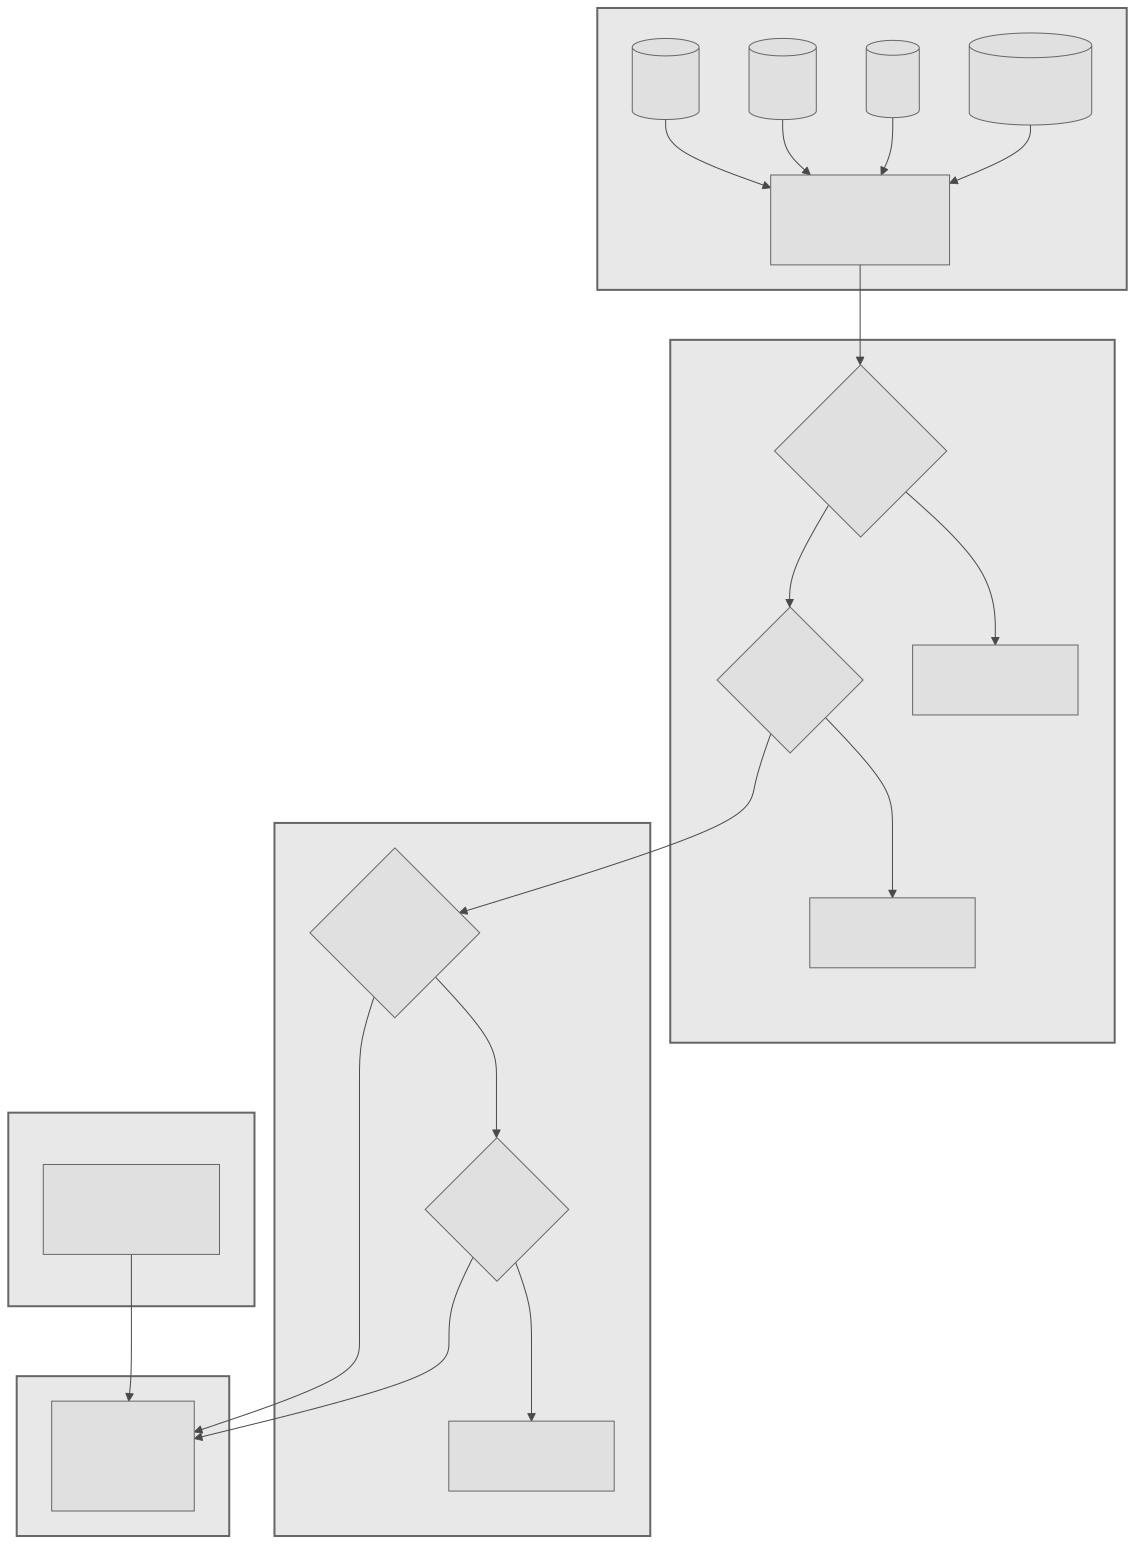
\includegraphics[width=0.9\textwidth,keepaspectratio]{figures/literature-flow.mmd.png}
\caption{Literature Selection Flow Diagram. The diagram shows the progression from initial database search (n ≈ 570) through title/abstract screening, full-text review, and quality assessment (AACODS for grey literature) to the final corpus of 135 sources (115 academic, 20 industry). Diagram source available in figures/literature-flow.mmd.}
\label{fig:literature-flow}
\end{figure}

\subsection{Stage 2: Screening and
Selection}\label{stage-2-screening-and-selection}

Sources were selected based on the following criteria:

\textbf{Inclusion Criteria:}

\begin{itemize}
\tightlist
\item
  Peer-reviewed publications in healthcare informatics, medical
  informatics, computer science, or health services research
\item
  Industry reports from established healthcare IT organizations (HIMSS,
  AHIMA, AMIA)
\item
  Publications from 2015-current, with emphasis on 2020-current for
  rapidly evolving NL2SQL technologies
\item
  English language publications
\item
  Sources with verifiable DOIs, URLs, or institutional attribution
\end{itemize}

\textbf{Exclusion Criteria:}

\begin{itemize}
\tightlist
\item
  Sources without verifiable attribution or institutional backing
\item
  Vendor marketing materials without independent validation
\item
  Preprints without subsequent peer-reviewed publication (exception:
  foundational NL2SQL benchmarks where peer review is pending)
\item
  Studies with unverifiable statistics or methodological concerns
\end{itemize}

\subsection{Stage 3: Quality
Assessment}\label{stage-3-quality-assessment}

Grey literature sources were assessed using the AACODS checklist
(\citeproc{ref-tyndall2010}{21}), which evaluates Authority, Accuracy,
Coverage, Objectivity, Date, and Significance. Sources with vendor
sponsorship were retained when no independent alternative existed but
flagged in-text. Table 2 summarizes the assessment.

\begin{longtable}[]{@{}
  >{\raggedright\arraybackslash}p{(\columnwidth - 10\tabcolsep) * \real{0.3200}}
  >{\raggedright\arraybackslash}p{(\columnwidth - 10\tabcolsep) * \real{0.2080}}
  >{\raggedright\arraybackslash}p{(\columnwidth - 10\tabcolsep) * \real{0.1920}}
  >{\raggedright\arraybackslash}p{(\columnwidth - 10\tabcolsep) * \real{0.1600}}
  >{\raggedright\arraybackslash}p{(\columnwidth - 10\tabcolsep) * \real{0.0800}}
  >{\raggedright\arraybackslash}p{(\columnwidth - 10\tabcolsep) * \real{0.0080}}@{}}
\caption{AACODS Assessment of Industry Sources.
\label{tbl:aacods}}\tabularnewline
\toprule\noalign{}
\begin{minipage}[b]{\linewidth}\raggedright
Source (Citation)
\end{minipage} & \begin{minipage}[b]{\linewidth}\raggedright
Authority / Accuracy
\end{minipage} & \begin{minipage}[b]{\linewidth}\raggedright
Coverage / Objectivity
\end{minipage} &
\multicolumn{3}{>{\raggedright\arraybackslash}p{(\columnwidth - 10\tabcolsep) * \real{0.2480} + 4\tabcolsep}@{}}{%
\begin{minipage}[b]{\linewidth}\raggedright
Date / Significance\textbar{} Include
\end{minipage}} \\
\midrule\noalign{}
\endfirsthead
\toprule\noalign{}
\begin{minipage}[b]{\linewidth}\raggedright
Source (Citation)
\end{minipage} & \begin{minipage}[b]{\linewidth}\raggedright
Authority / Accuracy
\end{minipage} & \begin{minipage}[b]{\linewidth}\raggedright
Coverage / Objectivity
\end{minipage} &
\multicolumn{3}{>{\raggedright\arraybackslash}p{(\columnwidth - 10\tabcolsep) * \real{0.2480} + 4\tabcolsep}@{}}{%
\begin{minipage}[b]{\linewidth}\raggedright
Date / Significance\textbar{} Include
\end{minipage}} \\
\midrule\noalign{}
\endhead
\bottomrule\noalign{}
\endlastfoot
HIMSS AMAM (\citeproc{ref-himss2024}{2}) & High† / Verifiable & Global /
High & 2024 / High & Yes & \\
Snowdon/HIMSS (\citeproc{ref-snowdon2024b}{22}) & High‡ / Verifiable &
N/A / High & 2024 / Medium & Yes & \\
Health Catalyst (\citeproc{ref-health2020}{23}) & Medium§ / Unverifiable
& US / Low & 2020 / Medium & Yes* & \\
Berkshire NHS (\citeproc{ref-berkshire2024}{24}) & High¶ / Verifiable &
Single site / High & 2024 / High & Yes & \\
Forrester/Microsoft (\citeproc{ref-forrester2024}{25}) & Medium∥ /
Unverifiable & Enterprise / Low♢ & 2024 / Medium & Yes* & \\
Oracle (\citeproc{ref-oracle2024}{26}) & Low§ / Unverifiable & N/A / Low
& 2024 / Low & Yes* & \\
Precedence Research (\citeproc{ref-precedence2024}{27}) & Medium\# /
Unverifiable & Global / Medium & 2024 / Medium & Yes & \\
Anthropic (\citeproc{ref-anthropic2025}{10}) & Medium§ / Verifiable &
N/A / Medium & 2025 / Low & Yes & \\
IBM Newsroom (\citeproc{ref-ibm2022}{28}) & High** / Verifiable & N/A /
High & 2022 / High & Yes & \\
CNBC/Haven (\citeproc{ref-lavito2021}{29}) & High** / Verifiable & N/A /
High & 2021 / High & Yes & \\
AHIMA/NORC (\citeproc{ref-american2023}{1}) & High†† / Verifiable & US /
High & 2023 / High & Yes & \\
\end{longtable}

†Industry standards body. ‡HIMSS officer. §Vendor. ¶NHS trust. ∥Analyst
firm. \#Market research. **Journalism. ††Professional association +
academic. ♢Sponsor. *Vendor sponsorship or low objectivity noted in
manuscript text.

\subsection{Stage 4: Synthesis and
Analysis}\label{stage-4-synthesis-and-analysis}

Reflecting the framework's iterative emergence from the literature,
evidence is synthesized thematically below:

\begin{enumerate}
\def\labelenumi{\arabic{enumi}.}
\tightlist
\item
  \textbf{Analytics maturity}: Evidence on HIMSS AMAM adoption,
  healthcare analytics capabilities, and organizational readiness
\item
  \textbf{Workforce turnover}: Evidence on nursing and IT staff turnover
  rates, institutional memory loss, and knowledge transfer challenges
\item
  \textbf{Technical barriers}: Evidence on NL2SQL benchmarks,
  healthcare-specific NLP challenges, and low-code implementation
  patterns
\end{enumerate}

This framework emerged iteratively from the literature rather than being
pre-specified, consistent with narrative review methodology.

\subsection{Methodological
Limitations}\label{methodological-limitations}

This narrative review has inherent limitations:

\begin{itemize}
\tightlist
\item
  \textbf{Non-exhaustive search}: Literature identification was
  selective rather than exhaustive; relevant studies may have been
  missed
\item
  \textbf{Limited formal quality assessment}: Grey literature sources
  were assessed using the AACODS checklist; however, no standardized
  quality assessment tool (e.g., GRADE, Cochrane Risk of Bias) was
  applied to peer-reviewed sources, as these tools are designed for
  clinical intervention studies rather than narrative reviews
\item
  \textbf{Single-coder bias risk}: Literature screening, data
  extraction, and thematic analysis were performed by a single author
  without independent verification. This introduces potential selection
  and interpretation bias that would be mitigated in systematic reviews
  through dual-coder protocols with inter-rater reliability assessment
\item
  \textbf{Post-hoc selection criteria}: Inclusion and exclusion criteria
  were refined during the review process rather than pre-registered
\item
  \textbf{No protocol registration}: This review was not registered in
  PROSPERO or similar registries
\item
  \textbf{Dated workforce statistics}: The primary healthcare IT
  turnover statistic (\textasciitilde34\% implied for new hires) derives
  from Ang and Slaughter's 2004 study (\citeproc{ref-ang2004}{7}). While
  recent surveys confirm workforce challenges persist
  (\citeproc{ref-american2023}{1}) and contemporary evidence suggests
  the situation may have worsened (55\% intent to leave among public
  health informatics specialists (\citeproc{ref-rajamani2025}{6})), no
  study has directly replicated the 2004 tenure measurement methodology.
  This paper reframes this ``data desert'' as evidence of the crisis
  itself: the industry is too unstable to track its own attrition
  effectively. Future research should address this methodological gap.
\end{itemize}

These limitations are balanced against the strengths of narrative review
methodology: ability to synthesize heterogeneous evidence types across
disciplinary boundaries, flexibility to pursue emerging themes, and
capacity to construct novel analytical frameworks that illuminate
connections between previously disconnected research domains.

\section{Framework Development and
Validation}\label{framework-development-and-validation}

This paper's primary contribution is the three-pillar analytical
framework for understanding healthcare analytics challenges: (1)
analytics maturity, (2) workforce agility, and (3) technical enablement.
This section documents the framework's development process and
theoretical grounding.

\subsection{Framework Development
Process}\label{framework-development-process}

The three-pillar framework emerged through iterative analysis of the
literature corpus. Initial review identified numerous disconnected
research streams: NL2SQL technical advances, HIMSS maturity models,
healthcare workforce turnover studies, knowledge management theory, and
healthcare IT implementation case studies. These appeared as isolated
topics until thematic analysis revealed recurring patterns of
interdependence.

The framework development followed these steps:

\begin{enumerate}
\def\labelenumi{\arabic{enumi}.}
\tightlist
\item
  \textbf{Theme Extraction}: Systematic coding of included sources
  identified recurring themes across technical, organizational, and
  workforce dimensions
\item
  \textbf{Pattern Recognition}: Cross-domain analysis revealed that
  challenges in each dimension amplified challenges in others. A root
  cause analysis (observation-why-repeat) determined the framework's
  ordering: low \textbf{Analytics Maturity} (Observation/Context) is
  driven by low \textbf{Workforce Agility} (Cause/Actor), which in turn
  is exacerbated by low \textbf{Technical Enablement} (Root
  Mechanism/Tool). This causal chain frames the three pillars, drawing
  on established RCA methodology for organizational learning
  (\citeproc{ref-allison2021}{30},\citeproc{ref-soylemez2017}{31}).
\item
  \textbf{Pillar Identification}: Three orthogonal yet interconnected
  dimensions emerged as the organizing structure:

  \begin{itemize}
  \tightlist
  \item
    \textbf{Analytics Maturity}: Organizational capability progression
    measured against HIMSS AMAM stages
  \item
    \textbf{Workforce Agility}: Human capital retention and tacit
    knowledge preservation
  \item
    \textbf{Technical Enablement}: NL2SQL capabilities and
    healthcare-specific implementation solutions
  \end{itemize}
\item
  \textbf{Framework Validation}: Pillar structure tested against the
  full corpus to confirm comprehensive coverage without significant gaps
\end{enumerate}

\subsection{Theoretical Grounding}\label{theoretical-grounding}

The three-pillar framework aligns with established models in healthcare
informatics and knowledge management:

\begin{table}[htbp]
\centering
\begin{tabular}{p{3cm}p{3.5cm}p{3.5cm}p{3.5cm}}
\toprule
\textbf{Three \newline Pillars} & \textbf{HIMSS AMAM Alignment} & \textbf{DIKW \newline Hierarchy} & \textbf{Knowledge Management} \\
\midrule
Analytics \newline Maturity & Stages 0-7 \newline Progression & Data \newline → Information & Organizational learning \\
Workforce \newline Agility & Implicit in \newline Advanced Stages & Knowledge (tacit) \newline → Wisdom & Tacit knowledge transfer \\
Technical \newline Enablement & Stage 6-7 \newline Requirements & Information \newline → Knowledge & Knowledge \newline Codification \\
\bottomrule
\end{tabular}
\caption{Framework Alignment with Established Models}
\label{tab:framework-alignment}
\end{table}

The HIMSS Analytics Maturity Assessment Model
(\citeproc{ref-himss2024}{2}) provides organizational benchmarks but
does not explicitly address workforce knowledge retention. The
Data-Information-Knowledge-Wisdom (DIKW) hierarchy
(\citeproc{ref-rowley2007}{32}) explains the progression from raw data
to actionable insight, but standard formulations do not address
institutional memory loss. The three-pillar framework synthesizes these
perspectives, positioning workforce dynamics as the critical enabler
connecting data access (analytics maturity) with organizational wisdom
(knowledge preservation). It draws on established knowledge management
theory for organizational learning
(\citeproc{ref-rao2006}{33},\citeproc{ref-massingham2018}{34}), tacit
knowledge transfer
(\citeproc{ref-farnese2019}{35},\citeproc{ref-foos2006}{36}), and
knowledge codification
(\citeproc{ref-benbya2004}{37},\citeproc{ref-zhang2025}{38}) to explain
these connections.

\subsection{Framework Scope and
Limitations}\label{framework-scope-and-limitations}

The framework is descriptive rather than prescriptive; it provides an
analytical lens for understanding healthcare analytics challenges but
does not mandate specific solutions. Future research should empirically
validate pillar interdependencies through longitudinal organizational
studies and develop quantitative metrics for framework dimensions.

\section{Literature Review: Evidence Across the Three
Pillars}\label{literature-review-evidence-across-the-three-pillars}

This narrative review synthesizes evidence across the three pillar
domains: analytics maturity, workforce agility, and technical enablement
(specifically natural language to SQL generation). Drawing from
peer-reviewed research, industry reports, and benchmark datasets
identified through the methodology described in Section 2 (Methodology),
we document the current state of each pillar and reveal
interconnections. Analysis reveals three critical findings: (1)
healthcare analytics maturity remains low with most organizations
struggling at basic stages, (2) healthcare workforce turnover creates
institutional memory loss that traditional approaches fail to address,
and (3) natural language to SQL generation has evolved significantly but
faces healthcare-specific challenges requiring specialized solutions.
Evidence across these three domains reveals significant interconnections
and compounding effects that the three-pillar framework synthesizes.

\subsection{State of Healthcare Analytics
Maturity}\label{state-of-healthcare-analytics-maturity}

\subsubsection{Low Organizational
Maturity}\label{low-organizational-maturity}

The Healthcare Information Management Systems Society (HIMSS) Analytics
Maturity Assessment Model (AMAM) provides the industry standard for
measuring analytics capabilities. Recent data reveals a concerning state
of analytics maturity in healthcare organizations globally
(\citeproc{ref-himss2024}{2}). The newly revised AMAM24 model, launched
in October 2024, represents a significant evolution from the original
framework.

Snowdon (\citeproc{ref-snowdon2024b}{22}), Chief Scientific Research
Officer at HIMSS, emphasizes that ``analytics as a discipline has
changed dramatically in the last five to 10 years,'' yet healthcare
organizations struggle to keep pace (\citeproc{ref-wang2018}{39}).
Research confirms healthcare's adoption of analytics often lags behind
other sectors such as retail and banking, partly due to the complexity
of implementing new technology in clinical environments
(\citeproc{ref-wang2018}{39}), (\citeproc{ref-wang2017}{40}). The newly
revised AMAM model shifts focus from technical capabilities to outcomes
and AI governance, requiring evidence of responsible algorithm
monitoring (\citeproc{ref-himss2024apac}{41}). This shift drove the
early 2025 validations of Tampa General Hospital and China Medical
University Hospital (CMUH) at Stage 7, confirming that AI readiness is
the new gatekeeper for analytics maturity
(\citeproc{ref-tgh2025}{42},\citeproc{ref-cmuh2025}{43}). Regional
adoption dynamics reveal distinct structural drivers: while North
American adoption is largely market-driven by value-based care, Middle
Eastern adoption is often characterized by government-mandated visions,
such as Saudi Arabia's centralized push for digital health excellence
which has propelled institutions like King Faisal Specialist Hospital to
Stage 7 (\citeproc{ref-ksa2024}{44}).

Quantitative evidence links organizational maturity to patient outcomes
through two related pathways. First, EMR adoption maturity provides
foundational infrastructure: cross-sectional studies using the HIMSS
Electronic Medical Record Adoption Model (EMRAM) demonstrate that
hospitals with advanced EMR adoption (levels 6-7) have 3.25 times higher
odds of achieving better Leapfrog Group Hospital Safety Grades compared
to hospitals at EMRAM level 0, with significantly reduced infection
rates and fewer adverse events (\citeproc{ref-snowdon2024}{45}).
Similarly, high-maturity hospitals have 1.8 to 2.24 times higher odds of
achieving higher patient experience ratings
(\citeproc{ref-snowdon2024a}{46}). Second, analytics capabilities build
on this digital foundation: big data analytics capabilities, combined
with complementary organizational resources and analytical personnel
skills, improve readmission rates and patient satisfaction
(\citeproc{ref-wang2019}{47}), while poor-quality data results in
diagnostic errors, ineffective treatments, and compromised patient care
(\citeproc{ref-gomes2025}{48}). Note that EMRAM measures EMR adoption
stages rather than analytics maturity directly; robust digital
infrastructure is a prerequisite for analytics, but the AMAM model
addresses the analytics-specific capability gap. However, evidence
explicitly linking the new AMAM framework to outcomes remains sparse.
Studies relying on older proxies yield mixed results: while some align
digital maturity with lower staff turnover and reduced errors
(\citeproc{ref-woods2024}{49}), others find no significant association
with readmission rates (\citeproc{ref-saintulysse2021}{50}) or mortality
(\citeproc{ref-martin2019}{51}), suggesting that maturity alone is
insufficient without workforce stability.

\subsubsection{Barriers to Analytics
Adoption}\label{barriers-to-analytics-adoption}

A systematic literature review of big data analytics in healthcare by
Kamble et al. (\citeproc{ref-kamble2019}{17}) identifies critical
barriers to analytics adoption. The study reveals that healthcare
enterprises struggle with technology selection, resource allocation, and
organizational readiness for data-driven decision making.

Health Catalyst's Healthcare Analytics Adoption Model
(\citeproc{ref-health2020}{23}), a vendor-produced framework,
corroborates these findings, documenting that most healthcare
organizations remain at Stages 0-3, characterized by:

\begin{itemize}
\tightlist
\item
  Fragmented data sources without integration
\item
  Limited automated reporting capabilities
\item
  Lack of standardized data governance
\item
  Minimal predictive or prescriptive analytics
\item
  Absence of real-time decision support
\end{itemize}

\subsubsection{The Analytics Skills Gap}\label{the-analytics-skills-gap}

The literature consistently identifies workforce capabilities as a
primary constraint. Healthcare organizations face mounting challenges in
extracting meaningful insights from the vast amount of unstructured
clinical text data generated daily (\citeproc{ref-navarro2023}{52}).
There is an acknowledged problem in health services where organizations
cannot make good use of available data due to a deficit in skilled
analysts across all sectors and levels
(\citeproc{ref-bardsley2016}{53}). Organizations face critical
challenges in recruiting and retaining professionals with the right
analytical skills, while the need for big data specialists with
analytical capabilities continues to grow
(\citeproc{ref-pesqueira2020}{54}). Traditional approaches to analytics
require extensive technical expertise and time that healthcare
professionals typically lack, creating a fundamental barrier to
analytics adoption (\citeproc{ref-american2023}{1}).

\subsubsection{Data Quality as a Barrier to Analytics
Maturity}\label{data-quality-as-a-barrier-to-analytics-maturity}

Beyond workforce constraints, data quality represents a fundamental
barrier preventing healthcare organizations from advancing their
analytics capabilities. Research consistently demonstrates that data
quality is both a prerequisite for and a dimension of analytics
maturity; organizations cannot progress to higher maturity stages
without first addressing data quality issues
(\citeproc{ref-carvalho2019}{55}). Multiple maturity frameworks,
including the Healthcare Data Quality Maturity Model (HDQM2) and the
Data Analytics Maturity Assessment Framework (DAMAF), explicitly
incorporate data quality as a core assessment dimension
(\citeproc{ref-pintovalverde2013}{56},\citeproc{ref-gokalp2023}{57}). A
cross-industry survey found that data management and quality issues,
including lack of documentation, accuracy, and consistency, continue to
challenge analytics organizations even as they mature, with the specific
challenges shifting from integration to privacy and documentation
concerns at higher maturity levels (\citeproc{ref-lismont2017}{58}).

The prevalence of data quality issues in healthcare databases is
substantial. A study of the National Cancer Database found missing data
rates ranging from 39.7\% for prostate cancer to 71.0\% for non-small
cell lung cancer (\citeproc{ref-yang2021}{59}). Medical registry data
shows 2.0\% to 4.6\% inaccurate records and 5\% to 6\% incomplete data
(\citeproc{ref-arts2002}{60}). Duplicate patient records affect 0.16\%
to 15.47\% of records across healthcare institutions, with wide
variation in management practices (\citeproc{ref-mccoy2013}{61}).
Analysis of Medicaid claims data found that 9.74\% of data cells
contained defects, with issues frequently remaining obscure due to
separation between data users and producers
(\citeproc{ref-zhang2024}{9}).

Critically, automated data quality tools alone are insufficient for
healthcare data. Research demonstrates that clinical domain expert
involvement is necessary at every stage of the data pipeline, including
curation, cleaning, and analysis (\citeproc{ref-rahman2020}{62}).
Automated tools fail to detect context-dependent errors such as mutually
exclusive values, definitional differences between institutions, or
plausibility issues that require clinical judgment
(\citeproc{ref-sirgo2018}{63}). Even successful automation requires
embedding clinical knowledge; generic automated cleaning tools from
other domains are unsuitable for clinical data, which requires
variable-specific rules based on clinical knowledge of normal ranges,
extreme values, and clinical contexts (\citeproc{ref-shi2021}{64}).

Compounding these challenges, healthcare database schemas are frequently
undocumented or poorly documented. Commercial EMR systems use
proprietary data models that are not publicly available, requiring
``detective work'' and reverse-engineering for research data integration
(\citeproc{ref-dugas2016}{65},\citeproc{ref-bokov2017}{66}). A
systematic review found that metadata models are often too complicated
for healthcare professionals without specific IT skills, resulting in
rare usage and poorly maintained documentation
(\citeproc{ref-ulrich2022}{67}). Poor chart documentation by healthcare
providers propagates downstream to administrative data quality issues
(\citeproc{ref-lucyk2017}{68}). Most critically, documentation knowledge
is lost with staff changes: decisions based on poorly documented data
represent significant costs and risks, with explicit identification of
``loss of information with staff changes'' as a key vulnerability
(\citeproc{ref-hovenga2013}{69}).

This creates a compounding effect across the three pillars: low-maturity
organizations have worse data quality and documentation, which requires
domain expertise to address, but that expertise is lost through
workforce turnover, further degrading data quality and preventing
maturity advancement. This persistent state of low maturity is not a
static condition but is actively driven by underlying workforce
dynamics, which the next section will explore.

\subsection{Healthcare Workforce Turnover and Knowledge
Loss}\label{healthcare-workforce-turnover-and-knowledge-loss}

\subsubsection{Turnover Rates and Financial
Impact}\label{turnover-rates-and-financial-impact}

While clinical turnover is well-studied
(\citeproc{ref-wu2024}{70},\citeproc{ref-ren2024}{71}), technical staff
turnover is more directly relevant to analytics maturity and carries
equally severe operational and financial consequences. Hong (2025)
demonstrates that turnover in federal IT roles directly degrades
organizational memory, causing a `sliding back' of performance
capabilities (\citeproc{ref-hong2025}{72}). This is compounded by
persistent vacancies; AHIMA/NORC (2023) report that 66\% of health
information professionals face staffing shortages, creating bottlenecks
that delay critical analytics initiatives
(\citeproc{ref-american2023}{1}).

The financial impact of this instability is substantial. Massingham
(2018) demonstrates that the total cost of knowledge loss in specialized
sectors can reach three times the annual salary budget for the departing
role (\citeproc{ref-massingham2018}{34}). In healthcare, vendor analysis
from Oracle (2024) corroborates this ``knowledge worker premium,''
documenting that turnover costs for informatics and innovation-focused
roles range from 1.5 to 2.0 times annual salary due to the extreme
scarcity of specialized digital skills (\citeproc{ref-oracle2024}{26}).
These figures align with established benchmarks for leadership
departures, where recruitment and lost productivity costs can exceed
\$500,000 per specialist (\citeproc{ref-willardgrace2019}{73}).

Technical and analytics staff face acute instability that extends beyond
general turnover baselines. While hospital-wide data establishes a high
churn environment, with 30\% of all new employees (clinical and
non-clinical) leaving within their first year
(\citeproc{ref-nsi2025}{74}), the crisis in informatics roles is even
more severe. Recent industry assessments reveal shortages at both
leadership and operational levels. Strategically, 53\% of healthcare
CIOs have held their current role for less than three years
(\citeproc{ref-wittkieffer2024}{4}), creating leadership vacuums that
disrupt long-term analytics initiatives. Operationally, this instability
is compounded by persistent vacancies, with 79\% of healthcare provider
organizations reporting shortages in ``Information and Digital Health''
roles (\citeproc{ref-himssworkforce2024}{5}). This creates a ``revolving
door'' for innovation-focused staff, significantly impacting the
continuity required for complex modernization. The 2023 AHIMA/NORC
workforce survey found that 66\% of health information professionals
report persistent staffing shortages, with 83\% reporting that unfilled
roles increased or remained stagnant over the past year
(\citeproc{ref-american2023}{1}).

The knowledge loss implications are substantial. Research documents
significant time-to-productivity requirements across healthcare IT
roles: basic EHR training requires 8 hours to 2 months for end-users,
while health information workforce development demands 18 months to 2
years for specialized roles (\citeproc{ref-ledikwe2013}{75}).
International Medical Informatics Association recommendations specify a
minimum of 1 year (60 ECTS credits) for biomedical and health
informatics specialists (\citeproc{ref-mantas2010}{76}), with
personalized EHR training programs requiring 6 months of blended
instruction to achieve meaningful competency improvements
(\citeproc{ref-musa2023}{77}). For IT developers and specialists,
research suggests up to 3 years are required to become fully fluent in
complex healthcare IT projects (\citeproc{ref-konrad2022}{78}). Given
that average tenures often fall below the three-year proficiency
threshold---with CIOs averaging less than three years and new technical
hires just 2.9 years
(\citeproc{ref-wittkieffer2024}{4},\citeproc{ref-ang2004}{7})---many
healthcare IT professionals spend only a limited portion of their
employment at full productivity and, in the case of IT developers, are
likely to leave before reaching full fluency. This creates a perpetual
cycle where organizations lose experienced staff before fully recouping
their training investment.

The impact on organizational capability is well-documented through the
lens of ``organizational forgetting.'' Rao and Argote (2006) establish
that high turnover rates disrupt the collective knowledge structures
required for complex task performance, effectively causing organizations
to ``forget'' established best practices (\citeproc{ref-rao2006}{33}).
This phenomenon is particularly acute in knowledge-intensive sectors;
Massingham (2018) demonstrates that the departure of experienced staff
leads to a measurable ``loss of competence'' that forces remaining teams
to regress to earlier learning stages
(\citeproc{ref-massingham2018}{34}). In the context of healthcare
analytics, this manifests not as immediate clinical errors, but as a
systemic inability to maintain the data quality and interpretive context
required for reliable decision-making.

\subsubsection{Institutional Memory
Loss}\label{institutional-memory-loss}

The concept of institutional memory in healthcare has received
increasing attention. Institutional memory encompasses the collective
knowledge, experiences, and expertise that enables organizational
effectiveness. Healthcare organizations typically lack formal mechanisms
for knowledge preservation, relying instead on person-to-person transfer
that fails during rapid turnover. Cultural and regulatory obstacles for
data sharing further limit the ability of healthcare organizations to
achieve the full potential of their data assets
(\citeproc{ref-mayo2016}{79}).

When experienced analysts, clinical informatics professionals, or
data-savvy clinicians leave, they take with them irreplaceable knowledge
about data definitions, business rules, analytical approaches, and
organizational context. Research on tacit knowledge transfer provides
strong evidence that this knowledge is inherently difficult to document
through traditional means. Empirical studies demonstrate that learning
related to tacit knowledge is often not captured in formal post-project
review reports (\citeproc{ref-goffin2011}{80}), and conventional
mechanisms such as documents, blueprints, and procedures fail because
tacit knowledge is not easily codified (\citeproc{ref-foos2006}{36}).
Research across multiple industries consistently shows that written
reports and databases fail to convey key learning from expert teams
(\citeproc{ref-goffin2010}{81}), while experts often lack the skills,
motivation, or time to document their expertise, and even when
documentation is attempted, essential aspects are lost due to lack of
shared experience between experts and novices
(\citeproc{ref-rintala2006}{82}).

\subsubsection{Inadequacy of Traditional
Approaches}\label{inadequacy-of-traditional-approaches}

The literature demonstrates that conventional knowledge management
approaches fail in healthcare contexts
(\citeproc{ref-shahbaz2019}{16},\citeproc{ref-mayo2016}{79}):

\begin{itemize}
\tightlist
\item
  Traditional knowledge transfer mechanisms show limited effectiveness
\item
  Organizations struggle to capture and maintain analytical expertise
\item
  Security concerns and employee resistance to change slow the pace of
  information system acceptance (\citeproc{ref-shahbaz2019}{16})
\item
  Person-to-person knowledge transfer fails during rapid turnover cycles
\end{itemize}

The failure of these traditional methods to preserve institutional
memory highlights the need for systemic solutions that can capture and
codify expertise at scale. Technical enablement, particularly through
modern AI and natural language interfaces, offers a potential mechanism
to address this gap, as the next section will discuss.

\subsection{State of Natural Language to SQL
Generation}\label{state-of-natural-language-to-sql-generation}

\subsubsection{Evolution and Technical
Advances}\label{evolution-and-technical-advances}

Recent systematic reviews document the rapid evolution of natural
language to SQL (NL2SQL) technologies. Ziletti and D'Ambrosi
(\citeproc{ref-ziletti2024}{20}) demonstrate that retrieval augmented
generation (RAG) approaches significantly improve query accuracy when
applied to electronic health records (EHRs), though they note that
``current language models are not yet sufficiently accurate for
unsupervised use'' in clinical settings. This assessment, based on 2024
models, has been challenged by late-2025 benchmarks showing GPT-5
exceeds physician baselines on standardized medical reasoning tasks
(\citeproc{ref-wang2025}{83},\citeproc{ref-openai2025}{84}), suggesting
the reasoning capabilities necessary for complex cohort definition are
now available, though human oversight remains recommended for safety.
Their work on the DE-SynPUF dataset shows that integrating medical
coding steps into the text-to-SQL process improves performance over
simple prompting approaches.

Benchmarking studies from 2024-2025
(\citeproc{ref-medagentbench2024}{85},\citeproc{ref-wu2024a}{86})
examining LLM-based systems for healthcare identify unique challenges:
medical terminology, characterized by abbreviations, synonyms, and
context-dependent meanings, remains a barrier to accurate query
generation. While previous models (GPT-4, Claude 3.5) achieved
\textasciitilde64-70\% accuracy on complex tasks, late-2025 models
demonstrate substantial improvements. GPT-5 achieves over 80\% accuracy
on complex medical reasoning benchmarks (\citeproc{ref-wang2025}{83}).
Crucially for analytics, on healthcare-specific NL2SQL tasks, GPT-5
achieves 64.6\% execution accuracy on the MIMICSQL dataset
(\citeproc{ref-blaskovic2025}{87}), while the HealthBench benchmark
shows hallucination rates of 0.7-1.0\%, representing a 4-6x improvement
over previous models (\citeproc{ref-openai2025}{84}).

\subsubsection{Healthcare-Specific
Challenges}\label{healthcare-specific-challenges}

The literature consistently identifies domain-specific obstacles in
healthcare NL2SQL implementation. A systematic review of NLP in EHRs
(\citeproc{ref-navarro2023}{52}) found that the lack of annotated data,
automated tools, and other challenges hinder the full utilization of NLP
for EHRs. The review, following PRISMA guidelines, categorized
healthcare NLP applications into seven areas, with information
extraction and clinical entity recognition proving most challenging due
to medical terminology complexity.

Wang et al. (\citeproc{ref-wang2020}{88}) demonstrate that healthcare
NL2SQL methods must move beyond the constraints of exact or string-based
matching to fully encompass the semantic complexities of clinical
terminology. This work emphasizes that general-purpose language models
fail to capture the nuanced relationships between medical concepts,
diagnoses codes (ICD), procedure codes (CPT), and medication
vocabularies (RxNorm).

\subsubsection{Promising Approaches and
Limitations}\label{promising-approaches-and-limitations}

Recent advances show promise in addressing these challenges. The
TREQS/MIMICSQL dataset development (\citeproc{ref-wang2020}{88}) and
EHRSQL benchmark (\citeproc{ref-lee2023}{89}) provide question-SQL pairs
specifically for healthcare, featuring questions in natural, free-form
language. Multi-modal benchmarks such as SM3-Text-to-Query
(\citeproc{ref-sivasubramaniam2024}{90}) extend evaluation beyond SQL to
support multiple query languages across diverse medical data
representations. This approach acknowledges that healthcare queries
often require multiple logical steps: population selection, temporal
relationships, aggregation statistics, and mathematical operations.

Healthcare-specific benchmarks continue to evolve alongside model
capabilities. The 2024 MedAgentBench evaluation found Claude 3.5 Sonnet
achieved 69.67\% success rate on medical agent tasks
(\citeproc{ref-medagentbench2024}{85}), (\citeproc{ref-wu2024a}{86});
subsequent 2025 benchmarks show GPT-5 significantly exceeding these
results, with the SCARE benchmark (\citeproc{ref-lee2025}{91}) providing
4,200 EHR question-SQL pairs across MIMIC-III, MIMIC-IV, and eICU
databases specifically designed to evaluate post-hoc safety mechanisms
for clinical text-to-SQL deployment. Graph-empowered approaches
combining LLMs with structured knowledge representations achieve 94.2\%
execution accuracy on MIMICSQL (\citeproc{ref-chen2025}{92}),
demonstrating that domain-specific architectural innovations can
substantially outperform general-purpose models. While these advances
narrow the gap between benchmark performance and clinical readiness,
domain-specific challenges in medical terminology and complex clinical
reasoning remain active research areas.

\subsubsection{Productivity and Efficiency
Evidence}\label{productivity-and-efficiency-evidence}

Emerging research documents quantifiable productivity gains from NL2SQL
implementations. In healthcare settings, organizations implementing
natural language interfaces report a 63\% increase in self-service
analytics adoption among non-technical staff and a 37\% reduction in
time spent on data retrieval tasks (\citeproc{ref-dadi2025}{93}).
Business analysts using these interfaces spend 42\% more time on
analysis rather than query construction (\citeproc{ref-dadi2025}{93}).

Clinical-specific natural language interfaces demonstrate significant
efficiency improvements. Criteria2Query, a natural language interface
for clinical database cohort definition, achieves fully automated query
formulation in an average of 1.22 seconds per criterion, enabling
researchers to query EHR data without mastering database query languages
(\citeproc{ref-yuan2019}{94}). The system has evolved through three
generations: the original rule-based approach
(\citeproc{ref-yuan2019}{94}), a human-machine collaboration version,
and Criteria2Query 3.0, which leverages GPT-4 to generate sharable
cohort identification queries against OMOP-CDM formatted databases
(\citeproc{ref-park2024}{95}). User studies show NL2SQL systems reduce
query completion times by 10-30\% compared to traditional SQL platforms
while improving accuracy from 50\% to 75\%, with users recovering from
errors 30-40 seconds faster (\citeproc{ref-ipeirotis2025}{96}).

The most substantial productivity gains appear in multimodal interfaces.
Research on speech-driven database querying demonstrates users can
specify SQL queries with an average speedup of 2.7x (up to 6.7x)
compared to traditional input methods, with user effort reduced by a
factor of 10x to 60x compared to raw typing
(\citeproc{ref-shah2020}{97}). Healthcare-specific natural language
query systems show dramatic improvements: a clinical data analytics
language (CliniDAL) reduced complex query formulation from ``many days''
with SQL to ``a few hours'' with natural language, with expert users
describing SQL as ``very tedious and time-consuming'' for the same
analytical tasks (\citeproc{ref-safari2014}{98}). NLP-driven data entry
systems have achieved 33\% time reduction with 15\% accuracy improvement
in clinical research settings (\citeproc{ref-han2019}{99}).
Healthcare-specific NL2SQL models such as MedT5SQL achieve 80.63\% exact
match accuracy on the MIMICSQL benchmark, demonstrating that
domain-adapted language models can effectively translate natural
language to SQL for clinical databases
(\citeproc{ref-marshan2024}{100}). These metrics provide peer-reviewed
evidence that complements vendor-sponsored efficiency claims.

Code modernization principles directly inform these productivity gains.
Foundational work on natural language interfaces to databases
(\citeproc{ref-hendrix1978}{11}) established that modular, decoupled
architecture enables effective NL access to legacy systems, a design
principle applied across subsequent research (e.g.,
(\citeproc{ref-saha2023}{101})). Modern implementations demonstrate that
retrieval-augmented generation (RAG) approaches reduce specialized
training requirements by 87.4\% compared to traditional querying methods
while achieving 92.3\% accuracy in interpreting business-specific
terminology from legacy mainframe records
(\citeproc{ref-khandelwal2025}{102}). This convergence of code
modernization and natural language interface technologies arises because
both rely on the same underlying large language models
(\citeproc{ref-ogunwole2023}{12}), (\citeproc{ref-arora2025}{13}),
suggesting that organizations investing in either capability
simultaneously advance both.

\subsection{Integration of Evidence: Synthesis Across Three
Pillars}\label{integration-of-evidence-synthesis-across-three-pillars}

\subsubsection{Pillar 1: Analytics Maturity and Democratized
Access}\label{pillar-1-analytics-maturity-and-democratized-access}

At its core, bridging technical and domain expertise serves a
fundamental patient care objective: enabling clinical professionals to
access and act on data that improves care quality. The convergence of
evidence reveals that traditional analytics maturity models often fail
because they assume a linear progression of \emph{technical} capability
rather than \emph{access} capability.

A critical distinction exists between traditional monitoring and dynamic
exploration. Visual dashboards excel at ``exploitation'' (monitoring
known metrics such as bed occupancy or infection rates) and provide
essential ``at-a-glance'' status (\citeproc{ref-health2020}{23}).
However, dashboards often create bottlenecks for novel or unanticipated
clinical questions, requiring a full build cycle and analyst
intervention (\citeproc{ref-syed2025}{103}). Conversational analytics
revolutionizes this ``time-to-insight'' by enabling ``exploration'' for
ad-hoc questions, reducing retrieval time from days to seconds
(\citeproc{ref-syed2025}{103}). Modern systems are increasingly moving
toward integrated ``Visual-Conversational'' interfaces, where natural
language simplifies complex, nested queries while visual panels align
with clinical workflow needs for analytical reasoning
(\citeproc{ref-samimi2025}{104},\citeproc{ref-ruoff2023}{105}). This
integration facilitates a fluid, iterative exploration that enhances
both information-finding effectiveness and clinical decision-making flow
(\citeproc{ref-chowdhury2020}{106}). User studies indicate that chatbot
proficiency can be reached after a single task repetition, suggesting a
lower training burden for high-agility enablement than traditional BI
dashboards (\citeproc{ref-holmes2019}{107}). By democratizing access,
organizations can advance their effective maturity, the ability to
actually use data, even while backend infrastructure remains in
transition.

\subsubsection{Pillar 2: Workforce Agility and Institutional
Memory}\label{pillar-2-workforce-agility-and-institutional-memory}

The literature suggests that effective knowledge preservation requires
active, embedded systems rather than passive documentation
(\citeproc{ref-benbya2004}{37},\citeproc{ref-whittaker2008}{108}). The
risk of institutional memory loss is not merely an HR issue but a
fundamental threat to analytics continuity (\citeproc{ref-rao2006}{33}).
When organizations choose to implement AI-based platforms, these can
serve as organizational memory systems by:

\begin{itemize}
\tightlist
\item
  Capturing decision-making patterns through usage
  (\citeproc{ref-moore2018}{109})
\item
  Encoding best practices in accessible formats
  (\citeproc{ref-zhang2025}{38})
\item
  Providing context-aware guidance to new users
\item
  Maintaining knowledge currency through continuous learning
\end{itemize}

These principles align with conversational AI approaches that embed
institutional knowledge within the AI model itself, making expertise
permanently accessible regardless of staff turnover
(\citeproc{ref-zhang2025}{38}). This directly addresses the Workforce
Agility pillar by decoupling organizational capability from individual
tenure. When a senior analyst leaves, their ``validated queries'' remain
in the system, allowing a junior replacement to immediately leverage
that expertise rather than starting from zero, mitigating the ``loss of
competence'' effect described by Massingham (2018)
(\citeproc{ref-massingham2018}{34}).

\subsubsection{Pillar 3: Technical Enablement as the
Catalyst}\label{pillar-3-technical-enablement-as-the-catalyst}

Technical enablement serves as the mechanism that breaks the compounding
cycle of low maturity and high turnover. Academic research provides
growing evidence for both conversational AI and low-code approaches as
effective catalysts in analytics workflows. In healthcare settings,
organizations implementing natural language interfaces report a 63\%
increase in self-service analytics adoption among non-technical staff
and a 37\% reduction in time spent on data retrieval tasks
(\citeproc{ref-dadi2025}{93}). Precision medicine platforms leveraging
conversational AI have demonstrated 92.5\% accuracy in parsing complex
biomedical queries, executing tasks faster than standard web portals
(\citeproc{ref-yang2025}{110}). Furthermore, experimental comparisons
show that natural language interfaces can accelerate database query
formulation by 2.7x to 6.7x compared to traditional methods
(\citeproc{ref-shah2020}{97}), reducing the dependency on specialized
technical staff.

Low-code platforms and conversational AI represent complementary
approaches to this enablement (\citeproc{ref-mogili2025}{111}). Low-code
platforms provide visual development environments that accelerate
application development and reduce coding requirements, while
conversational AI enables natural language interaction with data
systems. These approaches share core benefits: both democratize access
by enabling non-technical users to perform complex analyses previously
requiring data scientist intervention
(\citeproc{ref-berkshire2024}{24}), both accelerate development cycles
by abstracting technical complexity (\citeproc{ref-aveiro2023}{112}),
and both produce more self-documenting systems where business logic is
expressed in accessible formats rather than specialized code. Evidence
from low-code implementations thus informs conversational AI adoption,
as both address the same fundamental barrier: the gap between clinical
expertise and technical capability.

Healthcare-specific studies show concrete benefits: Pennington
(\citeproc{ref-pennington2023}{113}) found AI in revenue cycle
management accelerated payment cycles from 90 days to 40 days, while
Atobatele et al. (\citeproc{ref-atobatele2023}{114}) documented how
low-code platforms enable non-technical staff to build applications,
leading to efficiency gains. These findings collectively demonstrate
that technical enablement technologies produce measurable organizational
benefits not just by automating tasks, but by fundamentally changing
\emph{who} can perform them.

\subsection{Strategic Alignment with Industry
Trends}\label{strategic-alignment-with-industry-trends}

\subsubsection{Pillar 1 Alignment: Analytics Maturity
Trajectories}\label{pillar-1-alignment-analytics-maturity-trajectories}

Applied to recent industry literature, the three-pillar framework
highlights how barrier-reducing technologies track with broader
healthcare analytics trajectories. The revised HIMSS AMAM model
(\citeproc{ref-himss2024}{2}) emphasizes AI readiness and governance
frameworks, and conversational interfaces for analytics can be
understood as one illustrative application of these themes: they aim to
democratize access to data while preserving organizational controls,
rather than constituting a prescriptive pathway to maturity advancement.

\subsubsection{Pillar 2 Alignment: Workforce Knowledge
Risks}\label{pillar-2-alignment-workforce-knowledge-risks}

The literature emphasizes that institutional memory loss represents an
existential risk to healthcare analytics programs, particularly when
critical analytical practices remain tacit and concentrated in a small
number of experts. Within our three-pillar framework, this risk appears
as a compounding mechanism: workforce turnover erodes tacit expertise,
low analytics maturity limits organizations' ability to encode that
expertise, and technical barriers constrain efforts to make encoded
knowledge broadly accessible. Effective knowledge preservation therefore
requires mechanisms that transform tacit analytical knowledge into
encoded, shareable, and routinely accessible artifacts. This requirement
aligns with Nonaka's SECI model (Socialization, Externalization,
Combination, Internalization), which describes organizational knowledge
creation as a continuous dialogue between tacit and explicit knowledge
(\citeproc{ref-farnese2019}{35}). Recent research demonstrates that AI
tools, including conversational interfaces, can enhance all four SECI
stages, particularly facilitating the externalization process where
tacit analytical knowledge becomes explicit, queryable forms
(\citeproc{ref-zhang2025}{38}). This theoretical foundation supports
embedding organizational knowledge in systems rather than individuals,
ensuring continuity despite workforce turnover.

\subsubsection{Pillar 3 Alignment: Technical Enablement
ROI}\label{pillar-3-alignment-technical-enablement-roi}

Academic research documents multiple pathways to ROI for
barrier-reducing technologies in healthcare analytics. Conversational AI
implementations show direct benefits in analytical efficiency: Dadi et
al. (\citeproc{ref-dadi2025}{93}) report a 63\% increase in self-service
analytics adoption among non-technical staff and a 37\% reduction in
data retrieval time. Precision medicine platforms have demonstrated
92.5\% accuracy in parsing complex biomedical queries, executing tasks
significantly faster than standard web portals
(\citeproc{ref-yang2025}{110}). Furthermore, multimodal interfaces can
accelerate database query formulation by 2.7x to 6.7x compared to
traditional typing, reducing the cost of insight generation
(\citeproc{ref-shah2020}{97}). Pennington
(\citeproc{ref-pennington2023}{113}) documented that AI in revenue cycle
management accelerated payment cycles from 90 to 40 days, improving cash
flow through administrative analytics.

Low-code platform ROI provides analogous evidence for the value of
technical barrier reduction. Industry-sponsored research from Forrester
(\citeproc{ref-forrester2024}{25}) projects 206\% three-year ROI from
Power Platform implementations. Peer-reviewed studies corroborate these
findings: a systematic review identified cost and time reduction as the
most frequently discussed benefits across 17 studies
(\citeproc{ref-elkamouchi2023}{115}), healthcare institutions report
177\% ROI over 36 months with 67\% faster development
(\citeproc{ref-mogili2025}{111}), and small healthcare clinics document
250\% cumulative three-year ROI (\citeproc{ref-pervaiz2025}{116}). While
low-code and conversational AI differ in implementation approach, both
generate returns through the same mechanism: enabling domain experts to
accomplish tasks previously requiring specialized technical staff.
Market research supports continued investment in accessible analytics:
Precedence Research (\citeproc{ref-precedence2024}{27}) projects the
healthcare analytics market to grow from \$64.49 billion in 2025 to
\$369.66 billion by 2034 (21.41\% CAGR).

\subsection{Gaps in Current
Literature}\label{gaps-in-current-literature}

Despite substantial evidence supporting conversational AI in healthcare
analytics, several research gaps persist:

\begin{enumerate}
\def\labelenumi{\arabic{enumi}.}
\tightlist
\item
  \textbf{Long-term outcomes}: Most studies examine 6-24 month
  implementations
  (\citeproc{ref-dadi2025}{93},\citeproc{ref-pennington2023}{113});
  multi-year impacts remain understudied
\item
  \textbf{Scalability across specialties}: Evidence primarily focuses on
  general acute care
  (\citeproc{ref-wang2020}{88},\citeproc{ref-lee2023}{89});
  specialty-specific applications need investigation
\item
  \textbf{Governance frameworks}: Limited research on optimal governance
  models for democratized analytics
  (\citeproc{ref-himss2024}{2},\citeproc{ref-snowdon2024b}{22})
\item
  \textbf{Training methodologies}: Best practices for transitioning from
  traditional (\citeproc{ref-musa2023}{77}) to conversational analytics
  lack empirical validation
\item
  \textbf{Integration patterns}: Architectural guidance for
  incorporating conversational AI into existing healthcare IT ecosystems
  remains sparse
  (\citeproc{ref-park2024}{95},\citeproc{ref-yang2025}{110})
\item
  \textbf{Long-term productivity tracking}: While peer-reviewed studies
  now document immediate productivity gains (63\% self-service adoption
  increase, 37\% data retrieval time reduction, 10-30\% query completion
  time improvement (\citeproc{ref-yuan2019}{94}),
  (\citeproc{ref-dadi2025}{93}), (\citeproc{ref-shah2020}{97}),
  (\citeproc{ref-ipeirotis2025}{96})), longitudinal studies tracking
  sustained productivity improvements over multiple years remain limited
\item
  \textbf{Citizen developer productivity methodology}: No validated
  healthcare-specific instrument exists for measuring citizen developer
  productivity. While Berkshire NHS reports over 1,600 citizen
  developers (\citeproc{ref-berkshire2024}{24}), the methodology for
  quantifying their productivity contributions lacks standardization
  across studies
\item
  \textbf{AMAM-specific outcome evidence}: The HIMSS Analytics Maturity
  Assessment Model (AMAM) was released in October 2024; existing outcome
  studies linking maturity stages to patient outcomes use the older
  EMRAM (EHR adoption) model
  (\citeproc{ref-snowdon2024}{45},\citeproc{ref-snowdon2024a}{46}). As
  of this review, AMAM-specific outcome studies remain very limited,
  providing only emerging evidence for analytics maturity (as distinct
  from EHR adoption) impact on outcomes
\end{enumerate}

\subsection{Why the Problem Persists}\label{why-the-problem-persists}

Despite clear evidence of healthcare's analytics challenges and
available technology, the problem remains unsolved. Analysis of market
dynamics reveals three structural barriers:

\subsubsection{Failed Standardization
Approaches}\label{failed-standardization-approaches}

Large-scale efforts to standardize healthcare data and analytics have
consistently encountered fundamental barriers. Academic research
identifies a persistent tension between achieving short-term
institutional solutions and pursuing long-term global interoperability,
with standardization complexity arising from diverse community interests
and technical issues (\citeproc{ref-richesson2007}{117}). Data
standardization faces three primary technological obstacles: metadata
uncertainties, data transfer challenges, and missing data, compounded by
legacy data collection methods that have created a ``patchwork'' of
inconsistent organizational practices (\citeproc{ref-gal2019}{8}).

These challenges manifest in clinical practice through workflow
variability. Even within the same institution, clinical workflows vary
significantly, and transitions to standardized systems often cause
profound disruptions to existing processes
(\citeproc{ref-zheng2020}{118}). At the institutional level, data
fragmentation across different organizations creates barriers to
linkage, access, and care continuity, while governance issues including
unclear responsibilities and weak collaboration compound the problem
(\citeproc{ref-bogaert2021}{119}).

High-profile industry events illustrate these documented challenges. IBM
divested its Watson Health data and analytics assets to Francisco
Partners in 2022 (\citeproc{ref-ibm2022}{28}), following years of
underperformance attributed to a fundamental mismatch between AI
capabilities and clinical reality: the technology encountered the
``messy reality'' of healthcare data environments where centralized
models failed to account for the highly variable, institution-specific
business logic embedded in clinical workflows
(\citeproc{ref-strickland2019}{120},\citeproc{ref-yang2020}{121}).
Academic analysis identified additional contributing factors including
suboptimal business performance (only breaking even), a restrictive
top-down commercialization strategy that limited market reach, and the
highly-regulated nature of healthcare creating barriers to AI deployment
(\citeproc{ref-yang2020}{121}). The Haven healthcare venture (backed by
Amazon, Berkshire Hathaway, and JPMorgan Chase) disbanded in 2021 after
three years (\citeproc{ref-lavito2021}{29}), with academic analysis
identifying multiple contributing factors: even the three founding
companies could not effectively share health-care cost data with each
other, the venture never employed more than 75 people (limiting its
ability to effect industry-wide change), and leadership turnover
destabilized organizational continuity
(\citeproc{ref-acchiardo2021}{122}). Research on Big Tech platform entry
into healthcare positions both Watson Health and Haven within a broader
pattern of technology companies encountering regulatory complexity and
institutional resistance when attempting to standardize fragmented
healthcare systems (\citeproc{ref-ozalp2022}{123}). These outcomes align
with the academic literature's findings: standardized solutions face
significant barriers when applied across institutions with unique data
definitions, business rules, and clinical workflows.

These observations represent documented market events; however,
establishing causal mechanisms between organizational strategies and
interoperability outcomes requires controlled empirical research beyond
this review's scope. The patterns noted here warrant further
investigation through rigorous organizational studies.

\subsubsection{Deployment Constraint
Mismatch}\label{deployment-constraint-mismatch}

Healthcare organizations increasingly require solutions functional in
secure, network-isolated environments due to regulatory requirements and
data governance policies
(\citeproc{ref-nashid2023}{15},\citeproc{ref-bogaert2021}{119}).
General-purpose cloud AI services cannot meet these deployment
constraints while simultaneously lacking the institution-specific
context necessary for accurate analytics. The fundamental requirement
that institutional knowledge must be captured, preserved, and accessed
within each organization's specific environment cannot be addressed by
standardized cloud offerings
(\citeproc{ref-yang2020}{121},\citeproc{ref-ozalp2022}{123}).

These dynamics explain why, despite technological capability, the
healthcare analytics maturity gap persists. Solutions must be designed
for institution-specific deployment rather than cross-organizational
standardization.

\section{Discussion}\label{discussion}

\subsection{Strengths of the Evidence
Base}\label{strengths-of-the-evidence-base}

The evidence base for the three-pillar framework presents several
strengths:

\subsubsection{Benchmarked Data}\label{benchmarked-data}

The evidence base includes peer-reviewed benchmarking studies from top
venues (NEJM AI, NeurIPS, NAACL) that provide empirical validation of
LLM capabilities in healthcare contexts. Studies like MedAgentBench
(\citeproc{ref-medagentbench2024}{85}) and comprehensive medical LLM
evaluations (\citeproc{ref-wu2024a}{86}) offer reproducible,
quantitative performance metrics.

\subsubsection{Real-world
Implementations}\label{real-world-implementations}

The Berkshire Healthcare NHS Trust case
(\citeproc{ref-berkshire2024}{24}) demonstrates successful low-code
adoption in healthcare, with over 1,600 citizen developers creating
solutions. This provides concrete evidence that non-technical healthcare
professionals can effectively use these platforms.

\subsubsection{Interconnected
Challenges}\label{interconnected-challenges}

The framework illuminates how technical barriers, analytics maturity
constraints, and institutional memory loss compound each other,
explaining why single-pillar interventions often fail. This integrated
perspective enables healthcare organizations to understand why
addressing one challenge in isolation may not produce lasting
improvement.

\subsubsection{Economic Justification}\label{economic-justification}

The financial evidence is compelling, with Forrester Research
(\citeproc{ref-forrester2024}{25}) documenting 206\% three-year ROI from
low-code implementations. Market growth projections
(\citeproc{ref-precedence2024}{27}) showing the healthcare analytics
market expanding from \$64.49B to \$369.66B by 2034 indicate sustained
investment demand.

\subsubsection{Evidence Limitations}\label{evidence-limitations}

The evidence base includes important caveats. Ziletti and D'Ambrosi
(\citeproc{ref-ziletti2024}{20}) note that ``current language models are
not yet sufficiently accurate for unsupervised use,'' and benchmarking
studies (\citeproc{ref-ang2004}{7},\citeproc{ref-wu2024a}{86}) show
significant gaps between benchmark performance and clinical readiness.
This honest assessment enables appropriate implementation strategies.

\subsection{Limitations}\label{limitations}

Despite strong evidence supporting conversational AI adoption, several
limitations must be acknowledged:

\subsubsection{Implementation
Complexity}\label{implementation-complexity}

Healthcare environments present unique complexity challenges including
regulatory requirements, legacy system integration, and change
management across diverse user populations. Implementation timelines
reflect this complexity, though low-code approaches compare favorably to
traditional analytics infrastructure projects. Healthcare and
pharmaceutical organizations face particularly acute legacy
modernization challenges, paralleling patterns documented in broader
enterprise software contexts (\citeproc{ref-anthropic2025}{10}).

\subsubsection{Context-Specific Customization
Requirements}\label{context-specific-customization-requirements}

Healthcare organizations vary significantly in data structures, clinical
workflows, and analytical needs. Evidence suggests that successful
implementations require substantial customization to organizational
contexts, potentially limiting the applicability of standardized
approaches.

\subsubsection{Long-Term Outcome
Uncertainties}\label{long-term-outcome-uncertainties}

Most studies examine 6-24 month implementations. Questions remain about
long-term sustainability, user engagement over extended periods, and the
evolution of organizational capabilities beyond initial deployment
periods. The research gap analysis in the Literature Review identifies
this as a priority area for future investigation.

\subsubsection{Governance and Quality Assurance
Challenges}\label{governance-and-quality-assurance-challenges}

Democratizing analytics access creates new challenges in maintaining
data quality, analytical rigor, and clinical safety standards. While the
evidence shows reduced error rates with conversational AI, healthcare
organizations must develop new governance frameworks for managing
distributed analytical capabilities.

\subsubsection{Specialty-Specific Application
Gaps}\label{specialty-specific-application-gaps}

Evidence primarily focuses on general acute care settings. Applications
in specialized domains (oncology, cardiology, mental health) require
domain-specific validation and customization that may not generalize
from the existing evidence base.

\subsubsection{Methodological
Considerations}\label{methodological-considerations}

As a narrative review, this paper has methodological limitations
distinct from systematic reviews. The non-exhaustive literature search,
single-author synthesis, and post-hoc selection criteria may have
introduced selection or interpretation bias. No formal quality
assessment tool was applied to included studies. These limitations,
documented in detail in the Methodology section, should be considered
when interpreting findings. The transparency provided through explicit
documentation of search strategies, selection criteria, and synthesis
approach enables readers to assess potential biases and evaluate the
robustness of conclusions.

\subsection{Future Research
Directions}\label{future-research-directions}

The evidence review identifies several priority areas for future
investigation:

\subsubsection{Short-Term Research Priorities (\textless1
year)}\label{short-term-research-priorities-1-year}

\begin{enumerate}
\def\labelenumi{\arabic{enumi}.}
\tightlist
\item
  \textbf{Reference Implementation Validation}: Empirical validation of
  NL2SQL approaches using synthetic healthcare data (e.g., Synthea) in
  reproducible cloud environments, enabling benchmarking against
  established datasets (EHRSQL, MIMICSQL) without privacy constraints
\item
  \textbf{Schema Discovery for Healthcare Databases}: Research on
  automated primary/foreign key discovery algorithms applied to
  healthcare schemas, addressing the complexity of clinical data models
\item
  \textbf{Governance Framework Development}: Research on optimal
  governance models for democratized analytics
\item
  \textbf{Expansion to Unstructured Data}: While this paper focuses on
  SQL (structured data), \textasciitilde80\% of healthcare data is
  unstructured. Future research should explore how the three-pillar
  framework can provide the necessary governance structure for expansion
  into unstructured data via Vector/RAG technologies.
\end{enumerate}

\subsubsection{Medium-Term Research Priorities (1-2
years)}\label{medium-term-research-priorities-1-2-years}

\begin{enumerate}
\def\labelenumi{\arabic{enumi}.}
\tightlist
\item
  \textbf{Healthcare Terminology Integration}: Development of
  programmatic approaches for mapping natural language queries to
  standardized vocabularies (SNOMED CT, LOINC, RxNorm) within NL2SQL
  pipelines
\item
  \textbf{FHIR/OMOP Interoperability}: Research on reducing ETL burden
  for OMOP Common Data Model and FHIR transformations, enabling NL2SQL
  systems to operate across heterogeneous healthcare data standards
\item
  \textbf{Longitudinal Outcome Studies}: Multi-year implementations to
  assess sustained benefits and organizational evolution
\item
  \textbf{Comparative Effectiveness Research}: Head-to-head comparisons
  of different conversational AI approaches on healthcare-specific
  benchmarks
\end{enumerate}

\subsubsection{Long-Term Research Priorities (\textgreater2
years)}\label{long-term-research-priorities-2-years}

\begin{enumerate}
\def\labelenumi{\arabic{enumi}.}
\tightlist
\item
  \textbf{Organizational Transformation Studies}: Research on how
  conversational AI platforms reshape healthcare organizational
  capabilities
\item
  \textbf{Clinical Outcome Impact Assessment}: Studies linking improved
  analytics access to patient care outcomes
\item
  \textbf{Cross-Institution Knowledge Portals}: Investigation of
  federated approaches enabling knowledge sharing across healthcare
  organizations while maintaining privacy and security requirements
\end{enumerate}

\subsection{Illustrative Application: Knowledge Preservation
Mechanisms}\label{illustrative-application-knowledge-preservation-mechanisms}

To illustrate how the three-pillar framework might inform technology
design, we examine the validated query cycle concept introduced earlier.
This mechanism differs fundamentally from traditional knowledge
management approaches in healthcare. Traditional approaches rely on
documentation: analysts write procedures, create data dictionaries, and
maintain query libraries. However, documentation suffers from three
critical weaknesses: it becomes stale as systems evolve, it captures
procedural knowledge but not contextual judgment, and it requires active
maintenance that often lapses after staff transitions.

Validated query pairs address each weakness. First, validated pairs are
executable: they can be tested against current data to verify continued
correctness, unlike static documentation. Second, validated pairs
capture the complete mapping from business question to data retrieval
logic, embedding the contextual judgment that documentation typically
omits (why this join, why this filter, why this aggregation). To prevent
an intent gap, defined here as the loss of connection between the
original business question and its technical SQL implementation, a
validated pair is incomplete without mandatory ``Rationale Metadata,'' a
text field documenting \emph{why} the query was constructed in a
specific way (e.g., ``Excluding Hospice per 2025 CMS rules''). Third,
validation happens at the point of use rather than as a separate
maintenance task: every confirmed query becomes a knowledge artifact
without additional documentation effort.

This mechanism also differs from traditional query logging or usage
analytics. Query logs capture what was asked, but not whether the answer
was correct. Validated query pairs capture expert confirmation that the
SQL correctly answers the business question. This distinction is
critical for institutional memory: organizations need to know not just
what queries were run, but which queries produced trusted, verified
answers.

Governance requirements for the validated query cycle include: defining
who can validate queries (domain expertise requirements), establishing
validation workflows (review processes for high-stakes queries),
managing query versioning (as schemas evolve), and implementing
retrieval policies (when to return exact matches versus inform new
generation). Organizations implementing conversational AI platforms
should design these governance structures before deployment rather than
retrofitting them after knowledge accumulation begins.

\subsubsection{Resolving the Validator Paradox: Knowledge Ratchet and
Standard
Work}\label{resolving-the-validator-paradox-knowledge-ratchet-and-standard-work}

A critical paradox emerges in the proposed solution: reliance on expert
validation in an environment defined by expert turnover. If the experts
are leaving, who validates the AI? To resolve this ``validator
paradox,'' validation must be reframed not as \emph{eternal truth} but
as the ``standard work'' of informatics, drawing on Lean management
principles (\citeproc{ref-alukal2006}{124}).

In this model, a validated query represents the ``current best way'' to
perform an analysis. As Alukal and Manos
(\citeproc{ref-alukal2006}{124}) establish, standard work is the
prerequisite for Kaizen (continuous improvement): without a documented
standard, there is no baseline to improve upon. The Validated Query
Cycle functions as an ``organizational knowledge ratchet''
(\citeproc{ref-rao2006}{33}). Even provisional validation by mid-level
analysts captures operational logic into a procedural artifact. This
prevents the ``sliding back to zero'' that occurs during turnover,
allowing the organization to maintain a performance baseline that
persists independent of individual tenure (\citeproc{ref-hong2025}{72}).
Rather than requiring a permanent ``core nucleus'' of experts, the
system accumulates knowledge incrementally, using the structure of the
validation process to buffer against the disruptive effects of turnover.

\subsubsection{Comparative Analysis of Knowledge Preservation
Strategies}\label{comparative-analysis-of-knowledge-preservation-strategies}

Organizations have attempted to solve the institutional memory crisis
through various strategies. This review compares the proposed
conversational AI approach against established alternatives:

\begin{enumerate}
\def\labelenumi{\arabic{enumi}.}
\item
  \textbf{Code-Based Semantic Layers and Fabrics}: Traditional semantic
  layers (e.g., dbt, LookML) attempt to encode business logic in
  version-controlled repositories. However, research indicates these
  layers suffer from ``schema rot'' in healthcare environments where EMR
  data models change frequently (e.g., quarterly upgrades). The
  maintenance burden often exceeds the capacity of high-turnover teams,
  leading to misalignment between the layer and the underlying data
  (\citeproc{ref-mannapur2025}{125},\citeproc{ref-yupopa2005}{126}).
  Modern ``Semantic Fabrics'' using knowledge graphs and metadata-driven
  architectures (Data Governance 4.0) offer more flexible structures
  than relational databases
  (\citeproc{ref-oliveira2023}{127},\citeproc{ref-sivaranjani2025}{128}).
  AI-maintained adaptive frameworks can reduce false-positive quality
  alerts by 40\% under ``schema drift'' scenarios
  (\citeproc{ref-battula2025}{129}). However, the ``semantic gap''
  remains a fundamental challenge; medical concepts are inherently
  volatile, making stable References for programmers elusive
  (\citeproc{ref-lenz2007}{130}).
\item
  \textbf{Passive vs.~Active Capture}: Traditional knowledge management
  relies on passive capture (wikis, documentation) where users must stop
  working to document. Evidence suggests this negatively impacts
  participation and leads to inaccurate records due to cognitive load
  (\citeproc{ref-whittaker2008}{108}). In contrast, conversational
  interfaces represent active capture where the query itself is the
  documentation (\citeproc{ref-moore2018}{109}), integrating knowledge
  preservation directly into the analytical workflow.
\item
  \textbf{Governance vs.~Shadow IT}: Rigid, centralized models often
  drive analysts toward Shadow IT (extracting raw data to Excel) to
  achieve flexibility, defeating governance goals
  (\citeproc{ref-zimmermann2017}{131}). However, Shadow IT persists
  because it provides significant agility benefits, circumvents IT
  backlogs, and adds immediate value to business workgroups
  (\citeproc{ref-zimmermann2017}{131},\citeproc{ref-rivard1987}{132}).
  Spreadsheet-based components allow for rapid, local responsiveness to
  changing requirements (\citeproc{ref-kopper2020}{133}). Conversational
  interfaces offer a middle path: providing the flexibility and
  timeliness of Shadow IT within the governance perimeter of the
  validated query cycle (\citeproc{ref-oliveira2023}{127}). This
  approach aligns with recent evidence from UC Davis Health, where
  establishing standardized definitions enabled the organization to
  advance from AMAM Stage 0 to Stage 6 while weeding out biased AI
  models (\citeproc{ref-himss2025ucdavis}{134}). By decoupling data
  access from data definition, organizations can democratize the
  \emph{consumption} of analytics without democratizing the
  \emph{creation} of potentially flawed metrics.
\end{enumerate}

\subsubsection{Lifecycle Management: Continuous Analytic
Integration}\label{lifecycle-management-continuous-analytic-integration}

A validated SQL query is often treated as a static artifact, but in
healthcare, database schemas (Epic, Cerner, OMOP) change frequently,
breaking ``frozen'' code. To address ``Schema Drift,'' analytics must
adopt principles from software engineering: \textbf{Continuous Analytic
Integration}.

In this approach, Validated Query Pairs are managed not as wiki entries
but as software assets within a CI/CD pipeline. When the data warehouse
schema is updated (e.g., a quarterly EHR upgrade), the system
automatically re-runs the library of stored queries. Queries that fail
or return anomalous results are flagged for review. This transforms
``Institutional Memory'' from a stagnant repository into a living,
automated test suite that actively signals when organizational knowledge
has drifted from technical reality.

\subsection{Strategic Implications for Healthcare
Organizations}\label{strategic-implications-for-healthcare-organizations}

The evidence has implications for healthcare leaders considering
analytics strategy:

\subsubsection{Applying the Framework: A Three-Pillar
Assessment}\label{applying-the-framework-a-three-pillar-assessment}

The three-pillar framework provides a structured approach for
organizational self-assessment:

\paragraph{Pillar 1 Assessment: Analytics
Maturity}\label{pillar-1-assessment-analytics-maturity}

Where does the organization currently stand on the HIMSS AMAM scale?
What capabilities are needed to advance?

\paragraph{Pillar 2 Assessment: Workforce
Agility}\label{pillar-2-assessment-workforce-agility}

What tacit knowledge resides with individual staff members? How
vulnerable is the organization to knowledge loss through turnover?

\paragraph{Pillar 3 Assessment: Technical
Enablement}\label{pillar-3-assessment-technical-enablement}

What technical skills are currently required for data access? Which
clinical questions go unanswered due to access barriers?

\subsubsection{Three-Pillar Assessment
Rubric}\label{three-pillar-assessment-rubric}

The three-pillar framework enables organizational self-assessment to
determine readiness for and potential benefit from NL2SQL and
conversational AI interventions. Table 3 provides an evidence-based
rubric where each indicator anchors to reviewed literature.
Organizations scoring predominantly ``Higher Risk'' across pillars face
compounding challenges that NL2SQL platforms are specifically designed
to address: democratizing data access (Technical Barriers), preserving
institutional knowledge (Workforce Dynamics), and accelerating maturity
advancement (Analytics Maturity).

\textbf{Table 3: Three-Pillar Organizational Assessment Rubric}

\textbf{Pillar 1: Analytics Maturity}

\begin{longtable}[]{@{}
  >{\raggedright\arraybackslash}p{(\columnwidth - 8\tabcolsep) * \real{0.1392}}
  >{\raggedright\arraybackslash}p{(\columnwidth - 8\tabcolsep) * \real{0.2278}}
  >{\raggedright\arraybackslash}p{(\columnwidth - 8\tabcolsep) * \real{0.2658}}
  >{\raggedright\arraybackslash}p{(\columnwidth - 8\tabcolsep) * \real{0.2405}}
  >{\raggedright\arraybackslash}p{(\columnwidth - 8\tabcolsep) * \real{0.1266}}@{}}
\toprule\noalign{}
\begin{minipage}[b]{\linewidth}\raggedright
Indicator
\end{minipage} & \begin{minipage}[b]{\linewidth}\raggedright
Low Strength (1)
\end{minipage} & \begin{minipage}[b]{\linewidth}\raggedright
Medium Strength (2)
\end{minipage} & \begin{minipage}[b]{\linewidth}\raggedright
High Strength (3)
\end{minipage} & \begin{minipage}[b]{\linewidth}\raggedright
Evidence
\end{minipage} \\
\midrule\noalign{}
\endhead
\bottomrule\noalign{}
\endlastfoot
HIMSS AMAM Stage & Stages 0-2: Fragmented data, limited reporting &
Stages 3-4: Integrated warehouse, standardized definitions & Stages 5-7:
Predictive analytics, AI integration &
(\citeproc{ref-himss2024}{2},\citeproc{ref-health2020}{23}) \\
Self-service analytics & None; all analytics require IT intervention &
Partial; BI tools available but underutilized & Widespread; clinical
staff access data directly &
(\citeproc{ref-berkshire2024}{24},\citeproc{ref-wang2018}{39}) \\
AI/NL interface & No NL2SQL or conversational analytics & Pilot programs
or evaluation underway & Natural language query capability deployed &
(\citeproc{ref-ziletti2024}{20},\citeproc{ref-wang2020}{88}) \\
\end{longtable}

\textbf{Pillar 2: Workforce Agility}

\begin{longtable}[]{@{}
  >{\raggedright\arraybackslash}p{(\columnwidth - 8\tabcolsep) * \real{0.1392}}
  >{\raggedright\arraybackslash}p{(\columnwidth - 8\tabcolsep) * \real{0.2278}}
  >{\raggedright\arraybackslash}p{(\columnwidth - 8\tabcolsep) * \real{0.2658}}
  >{\raggedright\arraybackslash}p{(\columnwidth - 8\tabcolsep) * \real{0.2405}}
  >{\raggedright\arraybackslash}p{(\columnwidth - 8\tabcolsep) * \real{0.1266}}@{}}
\toprule\noalign{}
\begin{minipage}[b]{\linewidth}\raggedright
Indicator
\end{minipage} & \begin{minipage}[b]{\linewidth}\raggedright
Low Strength (1)
\end{minipage} & \begin{minipage}[b]{\linewidth}\raggedright
Medium Strength (2)
\end{minipage} & \begin{minipage}[b]{\linewidth}\raggedright
High Strength (3)
\end{minipage} & \begin{minipage}[b]{\linewidth}\raggedright
Evidence
\end{minipage} \\
\midrule\noalign{}
\endhead
\bottomrule\noalign{}
\endlastfoot
First-year Staff Turnover & \textgreater30\% (High Instability) &
15-30\% & \textless15\% (High Stability) &
(\citeproc{ref-nsi2025}{74}) \\
Leadership Stability (CIO) & Tenure \textless{} 3 years & Tenure 3-5
years & Tenure \textgreater{} 5 years &
(\citeproc{ref-wittkieffer2024}{4}) \\
Knowledge concentration & Critical expertise held by ≤3 individuals &
Partial documentation; some cross-training & Distributed expertise;
documented processes &
(\citeproc{ref-benbya2004}{37},\citeproc{ref-richesson2007}{117}) \\
Time-to-productivity & \textgreater18 months (specialized roles) & 6-18
months & \textless6 months with structured onboarding &
(\citeproc{ref-ledikwe2013}{75},\citeproc{ref-mantas2010}{76}) \\
Tacit knowledge capture & Person-dependent; undocumented tribal
knowledge & Partial documentation exists & Expertise embedded in
systems/AI & (\citeproc{ref-benbya2004}{37}) \\
\end{longtable}

\textbf{Pillar 3: Technical Enablement}

\begin{longtable}[]{@{}
  >{\raggedright\arraybackslash}p{(\columnwidth - 8\tabcolsep) * \real{0.1392}}
  >{\raggedright\arraybackslash}p{(\columnwidth - 8\tabcolsep) * \real{0.2278}}
  >{\raggedright\arraybackslash}p{(\columnwidth - 8\tabcolsep) * \real{0.2658}}
  >{\raggedright\arraybackslash}p{(\columnwidth - 8\tabcolsep) * \real{0.2405}}
  >{\raggedright\arraybackslash}p{(\columnwidth - 8\tabcolsep) * \real{0.1266}}@{}}
\toprule\noalign{}
\begin{minipage}[b]{\linewidth}\raggedright
Indicator
\end{minipage} & \begin{minipage}[b]{\linewidth}\raggedright
Low Strength (1)
\end{minipage} & \begin{minipage}[b]{\linewidth}\raggedright
Medium Strength (2)
\end{minipage} & \begin{minipage}[b]{\linewidth}\raggedright
High Strength (3)
\end{minipage} & \begin{minipage}[b]{\linewidth}\raggedright
Evidence
\end{minipage} \\
\midrule\noalign{}
\endhead
\bottomrule\noalign{}
\endlastfoot
Data access & SQL/technical expertise required for all queries & IT
queue for complex queries; basic self-service & Natural language or
visual query interfaces &
(\citeproc{ref-wang2018}{39},\citeproc{ref-pesqueira2020}{54}) \\
Interoperability & Fragmented systems; manual reconciliation required &
Partial integration; some automated feeds & Unified data platform;
real-time integration &
(\citeproc{ref-gal2019}{8},\citeproc{ref-bogaert2021}{119}) \\
Skills gap impact & Critical shortage preventing data utilization &
Acknowledged deficit with mitigation plans & Sufficient analysts across
departments &
(\citeproc{ref-bardsley2016}{53},\citeproc{ref-pesqueira2020}{54}) \\
\end{longtable}

\textbf{Multi-Pillar Convergence Assessment:}

\begin{longtable}[]{@{}
  >{\raggedright\arraybackslash}p{(\columnwidth - 4\tabcolsep) * \real{0.3333}}
  >{\raggedright\arraybackslash}p{(\columnwidth - 4\tabcolsep) * \real{0.2917}}
  >{\raggedright\arraybackslash}p{(\columnwidth - 4\tabcolsep) * \real{0.3750}}@{}}
\toprule\noalign{}
\begin{minipage}[b]{\linewidth}\raggedright
Organizational Profile
\end{minipage} & \begin{minipage}[b]{\linewidth}\raggedright
Framework Assessment
\end{minipage} & \begin{minipage}[b]{\linewidth}\raggedright
Implications for Analysis
\end{minipage} \\
\midrule\noalign{}
\endhead
\bottomrule\noalign{}
\endlastfoot
All pillars Low Strength & Self-reinforcing degradation cycle & All
three dimensions interact; comprehensive organizational assessment
warranted \\
1-2 pillars Low Strength & Compounding effects present & Framework
reveals interconnections requiring multi-dimensional analysis \\
All pillars High Strength & Continuous improvement stance & Monitor for
emerging challenges; single-pillar focus may suffice \\
\end{longtable}

The framework reveals why convergence matters: organizations facing
Higher Risk across multiple pillars experience compounding effects where
challenges in one domain exacerbate challenges in others. For example,
technical barriers that prevent knowledge capture interact with
workforce turnover to accelerate institutional memory loss, which in
turn degrades analytics maturity. This multi-pillar perspective explains
why single-domain interventions often produce limited results.

\subsubsection{Illustrative Application: Implementation
Patterns}\label{illustrative-application-implementation-patterns}

When organizations choose to apply the framework and evaluate
barrier-reducing technologies for potential adoption, implementation
evidence suggests several factors influence outcomes:

\begin{itemize}
\tightlist
\item
  \textbf{Governance Framework Development}: New policies and procedures
  for democratized analytics
\item
  \textbf{Change Management}: Training and support programs to ensure
  user adoption
\item
  \textbf{Phased Deployment}: Gradual rollout beginning with
  analytics-savvy early adopters
\item
  \textbf{Human Oversight}: Current NL2SQL limitations require
  maintaining human review of AI-generated outputs
  (\citeproc{ref-ziletti2024}{20})
\end{itemize}

\subsubsection{Mitigating ``Shadow IT'' with ``Golden
Queries''}\label{mitigating-shadow-it-with-golden-queries}

To prevent the ``chaos of conflicting definitions'' that can arise from
democratized analytics, organizations can introduce a ``Golden Query''
governance status. In this model, a central committee can certify
specific validated pairs as the ``source of truth'' for the
organization. This ensures that while many users can create and validate
queries, only a select few are designated as the official, trusted
queries for key metrics, thus mitigating the risks of ``Shadow IT.''

\section{Conclusion}\label{conclusion}

This narrative review synthesized evidence across three interconnected
domains: natural language to SQL generation, healthcare analytics
maturity, and workforce-driven institutional memory loss. The primary
contribution is a three-pillar analytical framework that reveals how
these challenges interconnect and compound each other.

\subsection{What the Framework
Reveals}\label{what-the-framework-reveals}

The three-pillar framework illuminates patterns that single-domain
analyses miss:

\begin{itemize}
\tightlist
\item
  \textbf{Analytics maturity gaps} leave clinical decisions unsupported
  by available data, and low maturity correlates with higher workforce
  turnover as staff leave organizations where they cannot accomplish
  their goals
\item
  \textbf{Workforce turnover} (\textasciitilde34\% implied annual rate
  for new healthcare IT staff as of 2004 (\citeproc{ref-ang2004}{7}))
  causes institutional memory loss that further degrades analytics
  capabilities, creating a reinforcing cycle
\item
  \textbf{Technical barriers} prevent organizations from capturing and
  preserving analytical knowledge, blocking recovery from either
  maturity gaps or turnover impacts
\end{itemize}

These interconnections explain why addressing any single pillar in
isolation often fails: improvements in one area erode when the
compounding effects from other pillars continue. The framework provides
a structured lens for organizational self-assessment.

\subsection{Summary of Contributions}\label{summary-of-contributions}

This narrative review contributes to healthcare informatics scholarship
through:

\begin{enumerate}
\def\labelenumi{\arabic{enumi}.}
\item
  \textbf{Three-Pillar Analytical Framework} (Primary Contribution): The
  framework synthesizes previously disconnected evidence from analytics
  maturity, workforce management, and natural language processing
  research, revealing how these capabilities interconnect and compound
  each other: low maturity accelerates turnover, turnover degrades
  agility, and low technical enablement prevents recovery from either.
\item
  \textbf{Evidence Synthesis}: We consolidate current evidence on each
  pillar, providing healthcare organizations with a comprehensive view
  of analytics maturity benchmarks, workforce turnover impacts, and
  NL2SQL technical capabilities in a single resource.
\item
  \textbf{Illustrative Application}: By applying established knowledge
  portal theory
  (\citeproc{ref-benbya2004}{37},\citeproc{ref-richesson2007}{117}), we
  describe the validated query cycle as one example of how the framework
  might inform technology design for institutional memory preservation.
\end{enumerate}

\subsection{Key Findings}\label{key-findings}

This review of academic and industry sources establishes several
critical findings:

\begin{enumerate}
\def\labelenumi{\arabic{enumi}.}
\item
  \textbf{Technical Progress with Limitations}: Natural language to SQL
  technologies have advanced significantly, with healthcare-specific
  benchmarks (\citeproc{ref-wang2020}{88},\citeproc{ref-lee2023}{89})
  demonstrating substantial progress in clinical NL2SQL tasks. However,
  current models are ``not yet sufficiently accurate for unsupervised
  use'' in clinical settings (\citeproc{ref-ziletti2024}{20}), requiring
  human oversight.
\item
  \textbf{Organizational Need}: Healthcare analytics maturity remains an
  ongoing challenge, with the revised HIMSS AMAM model
  (\citeproc{ref-himss2024}{2}) emphasizing the need for AI readiness
  and governance frameworks. Most organizations struggle to advance
  beyond basic reporting levels.
\item
  \textbf{Workforce Impact}: Healthcare IT staff new-hire turnover was
  implied at \textasciitilde34\% in 2004 (\citeproc{ref-ang2004}{7}),
  the highest instability among IT sectors at that time, and workforce
  challenges persist today (\citeproc{ref-american2023}{1}). Knowledge
  loss costs can reach three times annual salary budgets
  (\citeproc{ref-massingham2018}{34}), creating need for knowledge
  preservation approaches.
\item
  \textbf{Implementation Evidence}: Real-world implementations like
  Berkshire Healthcare NHS Trust (\citeproc{ref-berkshire2024}{24})
  demonstrate that low-code platforms can enable over 1,600 citizen
  developers in healthcare settings, with academic research documenting
  significant efficiency improvements and cost reductions
  (\citeproc{ref-sezgin2022}{135},\citeproc{ref-jiao2023}{136}).
\end{enumerate}

\subsection{Implications for Organizational
Assessment}\label{implications-for-organizational-assessment}

The evidence synthesis suggests healthcare organizations face decisions
that cannot be reduced to simple adoption/rejection binaries. Applying
\emph{primum non nocere} comprehensively requires organizational leaders
to:

\begin{enumerate}
\def\labelenumi{\arabic{enumi}.}
\item
  \textbf{Assess current harm exposure}: Quantify institutional memory
  loss from turnover, measure time-to-insight for clinical questions,
  and evaluate analytics capability gaps against organizational needs
\item
  \textbf{Evaluate intervention risks}: Consider NL2SQL accuracy
  limitations (``not yet sufficiently accurate for unsupervised use''
  (\citeproc{ref-ziletti2024}{20})), governance requirements, and
  implementation complexity
\item
  \textbf{Apply the three-pillar framework}: Use the analytics maturity,
  workforce agility, and technical enablement dimensions to structure
  organizational assessment and prioritization
\end{enumerate}

Throughout this assessment, quality patient care must remain the primary
metric. Operational efficiency, cost savings, and technical capabilities
are valuable only insofar as they advance healthcare's fundamental
mission.

This framework acknowledges that optimal decisions will vary by
organizational context. Healthcare systems with stable analytics teams
and mature data infrastructure face different risk profiles than those
experiencing rapid turnover and limited analytics capabilities. The
evidence does not prescribe universal solutions but provides structured
approaches for context-specific evaluation.

\subsection{Closing Reflection}\label{closing-reflection}

\emph{Primum non nocere} ultimately requires healthcare organizations to
make evidence-based judgments about both action and inaction. This
review contributes a three-pillar analytical framework to support those
judgments, synthesizing evidence on analytics maturity, workforce
dynamics, and technical capabilities.

The evidence does not prescribe universal adoption of any technology.
Rather, it establishes the scope and interconnection of challenges that
organizations must address through whatever means align with their
specific contexts, capabilities, and risk tolerances. The ongoing harms
documented in this review (institutional memory loss, analytics
capability gaps, and technical barriers to data access) merit the same
careful consideration as the risks of new technology adoption.

Healthcare's commitment to avoiding harm is best served by
evidence-based evaluation that considers all dimensions of potential
benefit and risk. The three-pillar framework offers one structured
approach for conducting such evaluations.

\section{Acknowledgments}\label{acknowledgments}

The author (S.T.H.) takes full responsibility for the final content,
conducted the research, and verified all claims and citations. Gemini
CLI (Gemini 3, Google) assisted with manuscript editing and refinement.
Figures were generated using the Mermaid graph language.

\section{Author Contributions}\label{author-contributions}

S.T.H. conceived the research, conducted the literature review, and
wrote the manuscript.

\section{Conflicts of Interest}\label{conflicts-of-interest}

The author declares the following competing interests: Samuel T Harrold
is a contract product advisor at Yuimedi, Inc., which develops
healthcare analytics software including conversational AI platforms
relevant to this review's subject matter. The author is also employed as
a Data Scientist at Indiana University Health. This paper presents an
analytical framework derived from published literature and does not
evaluate or recommend specific commercial products, including those of
the author's affiliated organizations. The views expressed are the
author's own and do not represent the official positions of Indiana
University Health or Yuimedi, Inc.

\section{Data Availability}\label{data-availability}

This is a narrative review synthesizing existing literature. No primary
datasets were generated or analyzed. All data cited are from publicly
available peer-reviewed publications and industry reports, referenced in
the bibliography. The literature search methodology and source selection
criteria are documented in the Methodology section.

\section{Code Availability}\label{code-availability}

Not applicable. No custom code was developed for this research.

\section{Funding}\label{funding}

Yuimedi provided funding for the author's time writing and researching
this manuscript.

\section{Abbreviations}\label{abbreviations}

AACODS: Authority, Accuracy, Coverage, Objectivity, Date, Significance
ACO: Accountable Care Organization AI: Artificial Intelligence AMAM:
Analytics Maturity Assessment Model CPT: Current Procedural Terminology
DAMAF: Data Analytics Maturity Assessment Framework DIKW:
Data-Information-Knowledge-Wisdom EHR: Electronic Health Record EMRAM:
Electronic Medical Record Adoption Model HDQM2: Healthcare Data Quality
Maturity Model HIMSS: Healthcare Information Management Systems Society
ICD: International Classification of Diseases IT: Information Technology
LLM: Large Language Model NL2SQL: Natural Language to SQL RAG:
Retrieval-Augmented Generation SQL: Structured Query Language

\section{References}\label{references}

\phantomsection\label{refs}
\begin{CSLReferences}{0}{1}
\bibitem[\citeproctext]{ref-american2023}
\CSLLeftMargin{1. }%
\CSLRightInline{NORC at the University of Chicago AHIMA \&. {Health
information workforce survey report} {[}Internet{]}. American Health
Information Management Association \& {NORC} at the University of
Chicago; 2023. Available from:
\url{https://www.ahima.org/news-publications/press-room-press-releases/2023-press-releases/health-information-workforce-shortages-persist-as-ai-shows-promise-ahima-survey-reveals/}}

\bibitem[\citeproctext]{ref-himss2024}
\CSLLeftMargin{2. }%
\CSLRightInline{Analytics H. {Analytics maturity assessment model (AMAM)
global report. Healthcare Information and Management Systems Society}
{[}Internet{]}. {HIMSS} Analytics; 2024. Available from:
\url{https://www.himss.org/maturity-models/amam/}}

\bibitem[\citeproctext]{ref-himss2024news}
\CSLLeftMargin{3. }%
\CSLRightInline{Healthcare IT News. {HIMSS launches modernised Analytics
Maturity Assessment Model} {[}Internet{]}. 2024. Available from:
\url{https://www.healthcareitnews.com/news/asia/himss24-apac-adoption-model-analytics-maturity-gets-facelift}}

\bibitem[\citeproctext]{ref-wittkieffer2024}
\CSLLeftMargin{4. }%
\CSLRightInline{WittKieffer. {CIO Insights: The State of Healthcare IT
Leadership} {[}Internet{]}. WittKieffer; 2024. Available from:
\url{https://api.wittkieffer.com/wp-content/uploads/2012/10/cio-insights-the-state-of-healthcare-it-leadership-wittkieffer-october-2024.pdf}}

\bibitem[\citeproctext]{ref-himssworkforce2024}
\CSLLeftMargin{5. }%
\CSLRightInline{HIMSS. {The Future of Workforce} {[}Internet{]}.
Healthcare Information; Management Systems Society; 2024. Available
from: \url{https://www.himss.org/resources/the-future-of-workforce/}}

\bibitem[\citeproctext]{ref-rajamani2025}
\CSLLeftMargin{6. }%
\CSLRightInline{Rajamani L S. {Public health informatics specialists in
state and local public health workforce: Insights from public health
workforce interests and needs survey}. Journal of Public Health
Management and Practice {[}Internet{]}. 2025; Available from:
\url{https://academic.oup.com/jpubhealth}}

\bibitem[\citeproctext]{ref-ang2004}
\CSLLeftMargin{7. }%
\CSLRightInline{Ang \&S S. {Turnover of information technology
professionals: The effects of internal labor market strategies}. {ACM}
{SIGMIS} Database: The {DATABASE} for Advances in Information Systems
{[}Internet{]}. 2004; Available from:
\url{https://dl.acm.org/doi/10.1145/1017114.1017118}}

\bibitem[\citeproctext]{ref-gal2019}
\CSLLeftMargin{8. }%
\CSLRightInline{Gal MS, Rubinfeld DL. {Data Standardization}. NYU Law
Review {[}Internet{]}. 2019;94(4):737--70. Available from:
\url{https://www.nyulawreview.org/issues/volume-94-number-4/data-standardization/}}

\bibitem[\citeproctext]{ref-zhang2024}
\CSLLeftMargin{9. }%
\CSLRightInline{Zhang Y, Callaghan-Koru JA, Koru G. {The challenges and
opportunities of continuous data quality improvement for healthcare
administration data}. JAMIA Open. 2024;7(2):ooae042. }

\bibitem[\citeproctext]{ref-anthropic2025}
\CSLLeftMargin{10. }%
\CSLRightInline{Anthropic. {Code modernization playbook: A practical
guide to modernizing legacy systems with {AI}} {[}Internet{]}. 2025.
Available from:
\url{https://resources.anthropic.com/code-modernization-playbook}}

\bibitem[\citeproctext]{ref-hendrix1978}
\CSLLeftMargin{11. }%
\CSLRightInline{Hendrix S G. G. {Developing a natural language interface
to complex data}. {ACM} Transactions on Database Systems {[}Internet{]}.
1978; Available from:
\url{https://dl.acm.org/doi/abs/10.1145/320251.320253}}

\bibitem[\citeproctext]{ref-ogunwole2023}
\CSLLeftMargin{12. }%
\CSLRightInline{Ogunwole \&O O. {Modernizing legacy systems: A scalable
approach to next-generation data architectures and seamless
integration}. International Journal of Multidisciplinary Research
{[}Internet{]}. 2023; Available from:
\url{https://www.allmultidisciplinaryjournal.com/uploads/archives/20250306182550_MGE-2025-2-018.1.pdf}}

\bibitem[\citeproctext]{ref-arora2025}
\CSLLeftMargin{13. }%
\CSLRightInline{Arora A. {Challenges of Integrating Artificial
Intelligence in Legacy Systems and Potential Solutions for Seamless
Integration}. {SSRN} {[}Internet{]}. 2025; Available from:
\url{https://papers.ssrn.com/sol3/papers.cfm?abstract_id=5268176}}

\bibitem[\citeproctext]{ref-latrella2024}
\CSLLeftMargin{14. }%
\CSLRightInline{Latrella \&B M. {Improving patient outcomes while
reducing readmissions with data analytics}. Management in Healthcare
{[}Internet{]}. 2024; Available from:
\url{https://www.ingentaconnect.com/content/hsp/mih/2024/00000008/00000004/art00006}}

\bibitem[\citeproctext]{ref-nashid2023}
\CSLLeftMargin{15. }%
\CSLRightInline{Nashid P S., Hossain MI. {Advanced Business Analytics in
Healthcare: Enhancing Clinical Decision Support and Operational
Efficiency}. Business and Social Sciences {[}Internet{]}.
2023;1(1):1--8. Available from:
\url{https://doi.org/10.25163/business.1110345}}

\bibitem[\citeproctext]{ref-shahbaz2019}
\CSLLeftMargin{16. }%
\CSLRightInline{Shahbaz G M. {Investigating the adoption of big data
analytics in healthcare: The moderating role of resistance to change}.
Journal of Big Data {[}Internet{]}. 2019; Available from:
\url{https://journalofbigdata.springeropen.com/articles/10.1186/s40537-019-0170-y}}

\bibitem[\citeproctext]{ref-kamble2019}
\CSLLeftMargin{17. }%
\CSLRightInline{Kamble G S. S. {A systematic perspective on the
applications of big data analytics in healthcare management}.
International Journal of Healthcare Management {[}Internet{]}. 2019;
Available from:
\url{https://www.tandfonline.com/doi/full/10.1080/20479700.2018.1531606}}

\bibitem[\citeproctext]{ref-bravorocca2023}
\CSLLeftMargin{18. }%
\CSLRightInline{Bravo Rocca GJ. Human-on-the-loop continual learning
{[}Internet{]} {[}PhD thesis{]}. Universitat Politècnica de Catalunya;
2023. Available from:
\url{https://www.tdx.cat/bitstream/handle/10803/695722/TGJBR1de1.pdf?sequence=1}}

\bibitem[\citeproctext]{ref-mosqueirarey2023}
\CSLLeftMargin{19. }%
\CSLRightInline{Mosqueira-Rey E et al. Human-in-the-loop machine
learning: A state of the art. Artificial Intelligence Review
{[}Internet{]}. 2023;56:3005--54. Available from:
\url{https://link.springer.com/content/pdf/10.1007/s10462-022-10246-w.pdf}}

\bibitem[\citeproctext]{ref-ziletti2024}
\CSLLeftMargin{20. }%
\CSLRightInline{Ziletti \&D A. {Retrieval augmented text-to-SQL
generation for epidemiological question answering using electronic
health records}. {NAACL} 2024 Clinical {NLP} Workshop {[}Internet{]}.
2024; Available from: \url{https://arxiv.org/abs/2403.09226}}

\bibitem[\citeproctext]{ref-tyndall2010}
\CSLLeftMargin{21. }%
\CSLRightInline{Tyndall J. {{AACODS} Checklist. Flinders University}
{[}Internet{]}. 2010. Available from:
\url{https://dspace.flinders.edu.au/jspui/bitstream/2328/3326/4/AACODS_Checklist.pdf}}

\bibitem[\citeproctext]{ref-snowdon2024b}
\CSLLeftMargin{22. }%
\CSLRightInline{Snowdon A. {New analytics maturity adoption model pushes
for digital transformation and data-driven decisions}. {HIMSS}
{[}Internet{]}. 2024; Available from:
\url{https://legacy.himss.org/news/new-analytics-maturity-adoption-model-pushes-digital-transformation-and-data-driven-decisions}}

\bibitem[\citeproctext]{ref-health2020}
\CSLLeftMargin{23. }%
\CSLRightInline{Catalyst H. {The healthcare analytics adoption model: A
roadmap to analytic maturity} {[}Internet{]}. 2020. Available from:
\url{https://www.healthcatalyst.com/learn/insights/healthcare-analytics-adoption-model-roadmap-analytic-maturity}}

\bibitem[\citeproctext]{ref-berkshire2024}
\CSLLeftMargin{24. }%
\CSLRightInline{Trust BHN. {Empowering citizen developers: Low-code
success in healthcare} {[}Internet{]}. 2024. Available from:
\url{https://ia.berkshirehealthcare.nhs.uk/citizen-developer-programme}}

\bibitem[\citeproctext]{ref-forrester2024}
\CSLLeftMargin{25. }%
\CSLRightInline{Research F. {The total economic impact of Microsoft
Power Apps. Forrester Consulting} {[}Internet{]}. 2024. Available from:
\url{https://tei.forrester.com/go/microsoft/powerappstei/?lang=en-us}}

\bibitem[\citeproctext]{ref-oracle2024}
\CSLLeftMargin{26. }%
\CSLRightInline{Oracle. {The real cost of turnover in healthcare}
{[}Internet{]}. 2024. Available from:
\url{https://www.oracle.com/human-capital-management/cost-employee-turnover-healthcare/}}

\bibitem[\citeproctext]{ref-precedence2024}
\CSLLeftMargin{27. }%
\CSLRightInline{Research P. {Healthcare analytics market size and
forecast 2025 to 2034} {[}Internet{]}. 2024. Available from:
\url{https://www.precedenceresearch.com/healthcare-analytics-market}}

\bibitem[\citeproctext]{ref-ibm2022}
\CSLLeftMargin{28. }%
\CSLRightInline{IBM. {Francisco Partners to Acquire IBM's Healthcare
Data and Analytics Assets}. {IBM} Newsroom {[}Internet{]}. 2022;
Available from:
\url{https://newsroom.ibm.com/2022-01-21-Francisco-Partners-to-Acquire-IBMs-Healthcare-Data-and-Analytics-Assets}}

\bibitem[\citeproctext]{ref-lavito2021}
\CSLLeftMargin{29. }%
\CSLRightInline{LaVito A. {Haven, the Amazon-Berkshire-JPMorgan venture
to disrupt healthcare, is disbanding after 3 years}. {CNBC}
{[}Internet{]}. 2021; Available from:
\url{https://www.cnbc.com/2021/01/04/haven-the-amazon-berkshire-jpmorgan-venture-to-disrupt-healthcare-is-disbanding-after-3-years.html}}

\bibitem[\citeproctext]{ref-allison2021}
\CSLLeftMargin{30. }%
\CSLRightInline{Allison DG, Peters H. {Root Cause Analysis (RCA) for the
Improvement of Healthcare Systems and Patient Safety}. CRC Press; 2021.
}

\bibitem[\citeproctext]{ref-soylemez2017}
\CSLLeftMargin{31. }%
\CSLRightInline{Soylemez M, Tarhan A. {A Review and Comparison of
Maturity/Capability Frameworks for Healthcare Process Assessment and
Improvement}. Software Quality Professional. 2017;19:28--42. }

\bibitem[\citeproctext]{ref-rowley2007}
\CSLLeftMargin{32. }%
\CSLRightInline{Rowley J.
\href{https://doi.org/10.1177/0165551506070706}{{The wisdom hierarchy:
representations of the DIKW hierarchy}}. Journal of Information Science.
2007;33(2):163--80. }

\bibitem[\citeproctext]{ref-rao2006}
\CSLLeftMargin{33. }%
\CSLRightInline{Rao RD, Argote L. Organizational learning and
forgetting: The effects of turnover and structure. European Management
Review {[}Internet{]}. 2006;3(2):77--85. Available from:
\url{https://onlinelibrary.wiley.com/doi/abs/10.1057/palgrave.emr.1500057}}

\bibitem[\citeproctext]{ref-massingham2018}
\CSLLeftMargin{34. }%
\CSLRightInline{Massingham PR. {Measuring the impact of knowledge loss:
A longitudinal study}. Journal of Knowledge Management {[}Internet{]}.
2018; Available from: \url{https://doi.org/10.1108/JKM-08-2016-0338}}

\bibitem[\citeproctext]{ref-farnese2019}
\CSLLeftMargin{35. }%
\CSLRightInline{Farnese B M. L. {Managing knowledge in organizations: A
Nonaka's {SECI} model operationalization}. Frontiers in Psychology
{[}Internet{]}. 2019; Available from:
\url{https://www.frontiersin.org/articles/10.3389/fpsyg.2019.02730}}

\bibitem[\citeproctext]{ref-foos2006}
\CSLLeftMargin{36. }%
\CSLRightInline{Foos S T. {Tacit knowledge transfer and the knowledge
disconnect}. Journal of Knowledge Management {[}Internet{]}. 2006;
Available from:
\url{https://www.emerald.com/insight/content/doi/10.1108/13673270610650067/full/html}}

\bibitem[\citeproctext]{ref-benbya2004}
\CSLLeftMargin{37. }%
\CSLRightInline{Benbya P H. {Corporate portal: A tool for knowledge
management synchronization}. International Journal of Information
Management {[}Internet{]}. 2004; Available from:
\url{https://doi.org/10.1016/j.ijinfomgt.2003.12.012}}

\bibitem[\citeproctext]{ref-zhang2025}
\CSLLeftMargin{38. }%
\CSLRightInline{Zhang D W. {{AI} challenges conventional knowledge
management: Light the way for reframing {SECI} model and Ba theory}.
Journal of Knowledge Management {[}Internet{]}. 2025; Available from:
\url{https://www.emerald.com/insight/content/doi/10.1108/JKM-03-2024-0262/full/html}}

\bibitem[\citeproctext]{ref-wang2018}
\CSLLeftMargin{39. }%
\CSLRightInline{Wang K Y., Byrd TA. {Big data analytics: Understanding
its capabilities and potential benefits for healthcare organizations}.
Technological Forecasting and Social Change {[}Internet{]}.
2018;126:3--13. Available from:
\url{https://www.sciencedirect.com/science/article/abs/pii/S0040162516000500}}

\bibitem[\citeproctext]{ref-wang2017}
\CSLLeftMargin{40. }%
\CSLRightInline{Wang \&H Y. {Exploring the path to big data analytics
success in healthcare}. Journal of Business Research {[}Internet{]}.
2017; Available from:
\url{https://www.sciencedirect.com/science/article/abs/pii/S0148296316304891}}

\bibitem[\citeproctext]{ref-himss2024apac}
\CSLLeftMargin{41. }%
\CSLRightInline{Healthcare IT News. {At HIMSS24 APAC, the Adoption Model
for Analytics Maturity gets facelift} {[}Internet{]}. 2024. Available
from:
\url{https://www.healthcareitnews.com/news/asia/himss24-apac-adoption-model-analytics-maturity-gets-facelift}}

\bibitem[\citeproctext]{ref-tgh2025}
\CSLLeftMargin{42. }%
\CSLRightInline{Tampa General Hospital. {Tampa General Hospital Awarded
Highest Designation in Analytics by HIMSS} {[}Internet{]}. 2025.
Available from:
\url{https://www.tgh.org/news/tgh-press-releases/2025/june/tampa-general-hospital-awarded-highest-designation-analytics-himss}}

\bibitem[\citeproctext]{ref-cmuh2025}
\CSLLeftMargin{43. }%
\CSLRightInline{China Medical University Hospital. {Taiwan's First
Hospital to Achieve AMAM Stage 7 Certification!} {[}Internet{]}. PR
Newswire; 2025. Available from:
\url{https://www.prnewswire.com/news-releases/taiwans-first-hospital-to-achieve-amam-stage-7-certification-302390824.html}}

\bibitem[\citeproctext]{ref-ksa2024}
\CSLLeftMargin{44. }%
\CSLRightInline{Medical Buyer. {2 medical groups in Saudi Arabia achieve
stage 7 digital maturity} {[}Internet{]}. 2024. Available from:
\url{https://medicalbuyer.co.in/2-medical-groups-in-saudi-arabia-achieve-stage-7-digital-maturity/}}

\bibitem[\citeproctext]{ref-snowdon2024}
\CSLLeftMargin{45. }%
\CSLRightInline{Snowdon H A., Wright A. {Digital maturity as a predictor
of quality and safety outcomes in {US} hospitals: Cross-sectional
observational study}. Journal of Medical Internet Research
{[}Internet{]}. 2024;26:e56316. Available from:
\url{https://www.jmir.org/2024/1/e56316}}

\bibitem[\citeproctext]{ref-snowdon2024a}
\CSLLeftMargin{46. }%
\CSLRightInline{Snowdon H A. {Digital maturity as a strategy for
advancing patient experience in {US} hospitals}. Journal of Patient
Experience {[}Internet{]}. 2024; Available from:
\url{https://journals.sagepub.com/doi/full/10.1177/23743735241253785}}

\bibitem[\citeproctext]{ref-wang2019}
\CSLLeftMargin{47. }%
\CSLRightInline{Wang K Y. {Leveraging big data analytics to improve
quality of care in healthcare organizations: A configurational
perspective}. British Journal of Management {[}Internet{]}. 2019;
Available from:
\url{https://onlinelibrary.wiley.com/doi/abs/10.1111/1467-8551.12332}}

\bibitem[\citeproctext]{ref-gomes2025}
\CSLLeftMargin{48. }%
\CSLRightInline{Gomes \&R J. {Evaluating maturity models in healthcare
information systems: A comprehensive review}. Healthcare {[}Internet{]}.
2025; Available from: \url{https://www.mdpi.com/2227-9032/13/1/1}}

\bibitem[\citeproctext]{ref-woods2024}
\CSLLeftMargin{49. }%
\CSLRightInline{Woods L, Eden R, Green D, Pearce A. {Impact of digital
health on the quadruple aims of healthcare: A correlational and
longitudinal study (Digimat Study)}. International Journal of Medical
Informatics {[}Internet{]}. 2024; Available from:
\url{https://www.sciencedirect.com/science/article/pii/S1386505624001916}}

\bibitem[\citeproctext]{ref-saintulysse2021}
\CSLLeftMargin{50. }%
\CSLRightInline{Saint-Ulysse C. {The Relationship between Hospitals'
Electronic Health Records Maturity and Excess Readmission Ratio}
{[}Internet{]}. Walden University Dissertations; 2021. Available from:
\url{https://scholarworks.waldenu.edu/cgi/viewcontent.cgi?article=12395&context=dissertations}}

\bibitem[\citeproctext]{ref-martin2019}
\CSLLeftMargin{51. }%
\CSLRightInline{Martin G, Clarke J, Liew F, Arora S, King D, Aylin P.
{Evaluating the impact of organisational digital maturity on clinical
outcomes in secondary care in England}. npj Digital Medicine
{[}Internet{]}. 2019; Available from:
\url{https://www.nature.com/articles/s41746-019-0118-9}}

\bibitem[\citeproctext]{ref-navarro2023}
\CSLLeftMargin{52. }%
\CSLRightInline{Navarro I D. F. {Clinical named entity recognition and
relation extraction using natural language processing of medical free
text: A systematic review}. International Journal of Medical Informatics
{[}Internet{]}. 2023; Available from:
\url{https://www.sciencedirect.com/science/article/pii/S1386505623001405}}

\bibitem[\citeproctext]{ref-bardsley2016}
\CSLLeftMargin{53. }%
\CSLRightInline{Bardsley M. {Understanding analytical capability in
health care: Do we have more data than insight? The Health Foundation}
{[}Internet{]}. 2016. Available from:
\url{https://www.health.org.uk/publications/understanding-analytical-capability-in-health-care}}

\bibitem[\citeproctext]{ref-pesqueira2020}
\CSLLeftMargin{54. }%
\CSLRightInline{Pesqueira S A. {Big data skills sustainable development
in healthcare and pharmaceuticals}. Journal of Medical Systems
{[}Internet{]}. 2020; Available from:
\url{https://link.springer.com/article/10.1007/s10916-020-01665-9}}

\bibitem[\citeproctext]{ref-carvalho2019}
\CSLLeftMargin{55. }%
\CSLRightInline{Carvalho J ildeao V, Rocha Á, Vasconcelos J.
\href{https://doi.org/10.1016/j.ijinfomgt.2018.07.001}{{A health data
analytics maturity model for hospitals information systems}}.
International Journal of Information Management. 2019;46:278--85. }

\bibitem[\citeproctext]{ref-pintovalverde2013}
\CSLLeftMargin{56. }%
\CSLRightInline{Pinto-Valverde J, Pérez-Guardado M. {HDQM2: healthcare
data quality maturity model}. In: Midwest association for information
systems conference. 2013. }

\bibitem[\citeproctext]{ref-gokalp2023}
\CSLLeftMargin{57. }%
\CSLRightInline{G"okalp MO, G"okalp E, G"okalp S. {The development of
data analytics maturity assessment framework: DAMAF}. Journal of
Software: Evolution and Process. 2023;35(4):e2448. }

\bibitem[\citeproctext]{ref-lismont2017}
\CSLLeftMargin{58. }%
\CSLRightInline{Lismont J, Vanthienen J, Baesens B, et al. {Defining
analytics maturity indicators: A survey approach}. International Journal
of Information Management. 2017;37(3):114--24. }

\bibitem[\citeproctext]{ref-yang2021}
\CSLLeftMargin{59. }%
\CSLRightInline{Yang DX, Khera R, Miccio JA, Jairam V, et al.
{Prevalence of missing data in the national cancer database and
association with overall survival}. JAMA Network Open.
2021;4(3):e211793. }

\bibitem[\citeproctext]{ref-arts2002}
\CSLLeftMargin{60. }%
\CSLRightInline{Arts DG, De Keizer NF, et al. {Defining and improving
data quality in medical registries: a literature review, case study, and
generic framework}. Journal of the American Medical Informatics
Association. 2002;9(6):600--11. }

\bibitem[\citeproctext]{ref-mccoy2013}
\CSLLeftMargin{61. }%
\CSLRightInline{McCoy AB, Wright A, Kahn MG, Shapiro JS, et al.
{Matching identifiers in electronic health records: implications for
duplicate records and patient safety}. BMJ Quality \& Safety.
2013;22(3):219--24. }

\bibitem[\citeproctext]{ref-rahman2020}
\CSLLeftMargin{62. }%
\CSLRightInline{Rahman P, Nandi A, Hebert C. {Amplifying domain
expertise in clinical data pipelines}. JMIR Medical Informatics.
2020;8(11):e19612. }

\bibitem[\citeproctext]{ref-sirgo2018}
\CSLLeftMargin{63. }%
\CSLRightInline{Sirgo G, Esteban F, Gómez J, Moreno G, et al.
{Validation of the ICU-DaMa tool for automatically extracting variables
for minimum dataset and quality indicators: The importance of data
quality assessment}. International Journal of Medical Informatics.
2018;112:166--72. }

\bibitem[\citeproctext]{ref-shi2021}
\CSLLeftMargin{64. }%
\CSLRightInline{Shi X, Prins C, Van Pottelbergh G, Mamouris P, et al.
{An automated data cleaning method for Electronic Health Records by
incorporating clinical knowledge}. BMC Medical Informatics and Decision
Making. 2021;21:1--12. }

\bibitem[\citeproctext]{ref-dugas2016}
\CSLLeftMargin{65. }%
\CSLRightInline{Dugas M, Neuhaus P, Meidt A, Doods J, Storck M, et al.
{Portal of medical data models: information infrastructure for medical
research and healthcare}. Database. 2016;2016. }

\bibitem[\citeproctext]{ref-bokov2017}
\CSLLeftMargin{66. }%
\CSLRightInline{Bokov AF, Bos AB, Manuel LS, et al. {Using prevalence
patterns to discover un-mapped flowsheet data in an electronic health
record data warehouse}. In: 2017 IEEE 30th international symposium on
computer-based medical systems (CBMS). IEEE; 2017. p. 509--14. }

\bibitem[\citeproctext]{ref-ulrich2022}
\CSLLeftMargin{67. }%
\CSLRightInline{Ulrich H, Kock-Schoppenhauer AK, et al. {Understanding
the nature of metadata: systematic review}. Journal of Medical Internet
Research. 2022;24(1):e25440. }

\bibitem[\citeproctext]{ref-lucyk2017}
\CSLLeftMargin{68. }%
\CSLRightInline{Lucyk K, Tang K, Quan H. {Barriers to data quality
resulting from the process of coding health information to
administrative data: a qualitative study}. BMC Health Services Research.
2017;17(1):1--10. }

\bibitem[\citeproctext]{ref-hovenga2013}
\CSLLeftMargin{69. }%
\CSLRightInline{Hovenga EJ, Grain H. {Health data and data governance}.
In: Health information governance in a digital environment. IOS Press;
2013. p. 67--94. }

\bibitem[\citeproctext]{ref-wu2024}
\CSLLeftMargin{70. }%
\CSLRightInline{Wu L F., Li L. {Worldwide prevalence and associated
factors of nursing staff turnover: A systematic review and
meta-analysis}. Nursing Open {[}Internet{]}. 2024;11:e2097. Available
from: \url{https://pmc.ncbi.nlm.nih.gov/articles/PMC10802134/}}

\bibitem[\citeproctext]{ref-ren2024}
\CSLLeftMargin{71. }%
\CSLRightInline{Ren W L. {Global prevalence of nurse turnover rates: A
meta-analysis of 21 studies from 14 countries}. Journal of Nursing
Management {[}Internet{]}. 2024; Available from:
\url{https://pmc.ncbi.nlm.nih.gov/articles/PMC11919231/}}

\bibitem[\citeproctext]{ref-hong2025}
\CSLLeftMargin{72. }%
\CSLRightInline{Hong JH. When does employee turnover matter?
Organizational memory in federal IT. Journal of Public Administration
Research and Theory {[}Internet{]}. 2025; Available from:
\url{https://academic.oup.com/jpart/advance-article-abstract/doi/10.1093/jopart/muaf019/8162522}}

\bibitem[\citeproctext]{ref-willardgrace2019}
\CSLLeftMargin{73. }%
\CSLRightInline{Willard-Grace K R. {Burnout and health care workforce
turnover}. The Annals of Family Medicine {[}Internet{]}. 2019; Available
from: \url{https://www.annfammed.org/content/17/1/36}}

\bibitem[\citeproctext]{ref-nsi2025}
\CSLLeftMargin{74. }%
\CSLRightInline{NSI Nursing Solutions. {2025 National Health Care
Retention \& RN Staffing Report} {[}Internet{]}. NSI Nursing Solutions;
2024. Available from:
\url{https://www.nsinursingsolutions.com/documents/library/nsi_national_health_care_retention_report.pdf}}

\bibitem[\citeproctext]{ref-ledikwe2013}
\CSLLeftMargin{75. }%
\CSLRightInline{Ledikwe R J. H. {Establishing a health information
workforce: Innovation for low- and middle-income countries}. Human
Resources for Health {[}Internet{]}. 2013; Available from:
\url{https://human-resources-health.biomedcentral.com/articles/10.1186/1478-4491-11-35}}

\bibitem[\citeproctext]{ref-mantas2010}
\CSLLeftMargin{76. }%
\CSLRightInline{Mantas A J. {Recommendations of the International
Medical Informatics Association (IMIA) on education in biomedical and
health informatics: First revision}. Methods of Information in Medicine
{[}Internet{]}. 2010; Available from:
\url{https://pubmed.ncbi.nlm.nih.gov/20054502/}}

\bibitem[\citeproctext]{ref-musa2023}
\CSLLeftMargin{77. }%
\CSLRightInline{Musa D S. {The impact of training on electronic health
records related knowledge, practical competencies, and staff
satisfaction: A pre-post intervention study among wellness center
providers in a primary health-care facility}. Journal of
Multidisciplinary Healthcare {[}Internet{]}. 2023; Available from:
\url{https://pmc.ncbi.nlm.nih.gov/articles/PMC10243608/}}

\bibitem[\citeproctext]{ref-konrad2022}
\CSLLeftMargin{78. }%
\CSLRightInline{Konrad \&S I. {Exploring the potential of an {IT}
capability in its bootstrap phase from a task driven onboarding
perspective: Insights toward information infrastructure in healthcare}
{[}Internet{]} {[}Master's thesis{]}. 2022. Available from:
\url{https://www.diva-portal.org/smash/record.jsf?pid=diva2:1684142}}

\bibitem[\citeproctext]{ref-mayo2016}
\CSLLeftMargin{79. }%
\CSLRightInline{Mayo D C. S. {How can we effect culture change toward
data-driven medicine?} International Journal of Radiation Oncology,
Biology, Physics {[}Internet{]}. 2016; Available from:
\url{https://www.redjournal.org/article/S0360-3016(16)00260-1/fulltext}}

\bibitem[\citeproctext]{ref-goffin2011}
\CSLLeftMargin{80. }%
\CSLRightInline{Goffin \&K K. {Tacit knowledge, lessons learnt, and new
product development}. Journal of Product Innovation Management
{[}Internet{]}. 2011; Available from:
\url{https://onlinelibrary.wiley.com/doi/abs/10.1111/j.1540-5885.2010.00798.x}}

\bibitem[\citeproctext]{ref-goffin2010}
\CSLLeftMargin{81. }%
\CSLRightInline{Goffin K K. {Managing lessons learned and tacit
knowledge in new product development}. Research-Technology Management
{[}Internet{]}. 2010; Available from:
\url{https://www.tandfonline.com/doi/abs/10.1080/08956308.2010.11657637}}

\bibitem[\citeproctext]{ref-rintala2006}
\CSLLeftMargin{82. }%
\CSLRightInline{Rintala \&H N. {Methods for sharing tacit nuclear
knowledge and expertise}. International Journal of Nuclear Knowledge
Management {[}Internet{]}. 2006; Available from:
\url{https://www.inderscienceonline.com/doi/abs/10.1504/IJNKM.2006.009880}}

\bibitem[\citeproctext]{ref-wang2025}
\CSLLeftMargin{83. }%
\CSLRightInline{Wang H S. {Capabilities of GPT-5 on multimodal medical
reasoning}. arXiv preprint {[}Internet{]}. 2025; Available from:
\url{https://arxiv.org/abs/2508.08224}}

\bibitem[\citeproctext]{ref-openai2025}
\CSLLeftMargin{84. }%
\CSLRightInline{OpenAI. {HealthBench: A benchmark for evaluating LLMs in
healthcare}. arXiv preprint {[}Internet{]}. 2025; Available from:
\url{https://arxiv.org/abs/2505.08775}}

\bibitem[\citeproctext]{ref-medagentbench2024}
\CSLLeftMargin{85. }%
\CSLRightInline{Jiang B Y., Chen JH. {MedAgentBench: A virtual {EHR}
environment to benchmark medical {LLM} agents}. {NEJM} {AI}
{[}Internet{]}. 2025; Available from:
\url{https://ai.nejm.org/doi/full/10.1056/AIdbp2500144}}

\bibitem[\citeproctext]{ref-wu2024a}
\CSLLeftMargin{86. }%
\CSLRightInline{Wu Q C., Xie W. {Towards evaluating and building
versatile large language models for medicine}. npj Digital Medicine
{[}Internet{]}. 2025; Available from:
\url{https://www.nature.com/articles/s41746-024-01390-4}}

\bibitem[\citeproctext]{ref-blaskovic2025}
\CSLLeftMargin{87. }%
\CSLRightInline{Blašković T L., Lorencin I. {Robust clinical querying
with local LLMs: Lexical challenges in NL2SQL and RAG-QA on EHRs}. Big
Data and Cognitive Computing {[}Internet{]}. 2025;9(10):256. Available
from: \url{https://www.mdpi.com/2504-2289/9/10/256}}

\bibitem[\citeproctext]{ref-wang2020}
\CSLLeftMargin{88. }%
\CSLRightInline{Wang S P. {Text-to-SQL generation for question answering
on electronic medical records}. In: Proceedings of the web conference
2020 {[}Internet{]}. 2020. Available from:
\url{https://arxiv.org/abs/1908.01839}}

\bibitem[\citeproctext]{ref-lee2023}
\CSLLeftMargin{89. }%
\CSLRightInline{Lee et al G. {EHRSQL: A practical text-to-SQL benchmark
for electronic health records}. In: Proceedings of NeurIPS 2022
{[}Internet{]}. 2023. Available from:
\url{https://arxiv.org/abs/2301.07695}}

\bibitem[\citeproctext]{ref-sivasubramaniam2024}
\CSLLeftMargin{90. }%
\CSLRightInline{Sivasubramaniam OA S. {SM3-Text-to-Query: Synthetic
multi-model medical text-to-query benchmark}. Advances in Neural
Information Processing Systems {[}Internet{]}. 2024; Available from:
\url{https://arxiv.org/abs/2411.05521}}

\bibitem[\citeproctext]{ref-lee2025}
\CSLLeftMargin{91. }%
\CSLRightInline{Lee C G. {SCARE: A benchmark for {SQL} correction and
question answerability classification for reliable {EHR} question
answering}. arXiv preprint {[}Internet{]}. 2025; Available from:
\url{https://arxiv.org/abs/2511.17559}}

\bibitem[\citeproctext]{ref-chen2025}
\CSLLeftMargin{92. }%
\CSLRightInline{Chen P Q. {Graph-empowered text-to-SQL generation on
electronic medical records}. Pattern Recognition {[}Internet{]}. 2025;
Available from:
\url{https://www.sciencedirect.com/science/article/pii/S0031320324008197}}

\bibitem[\citeproctext]{ref-dadi2025}
\CSLLeftMargin{93. }%
\CSLRightInline{Dadi CB, Hoque MR, Ali MM, Ferdausi S, Fatema K, Hasan
MR. {Natural Language Interfaces for Database Management: Bridging the
Gap Between Users and Data through Conversational {AI}}. Journal of
Computer Science and Technology Studies {[}Internet{]}.
2025;7(3):927--33. Available from:
\url{https://al-kindipublisher.com/index.php/jcsts/article/view/9694}}

\bibitem[\citeproctext]{ref-yuan2019}
\CSLLeftMargin{94. }%
\CSLRightInline{Yuan R C. {Criteria2Query: a natural language interface
to clinical databases for cohort definition}. Journal of the American
Medical Informatics Association {[}Internet{]}. 2019; Available from:
\url{https://academic.oup.com/jamia/article-abstract/26/4/294/5308980}}

\bibitem[\citeproctext]{ref-park2024}
\CSLLeftMargin{95. }%
\CSLRightInline{Park F J. {Criteria2Query 3.0: Leveraging generative
large language models for clinical trial eligibility query generation}.
Journal of Biomedical Informatics {[}Internet{]}. 2024; Available from:
\url{https://www.sciencedirect.com/science/article/pii/S1532046424000650}}

\bibitem[\citeproctext]{ref-ipeirotis2025}
\CSLLeftMargin{96. }%
\CSLRightInline{Ipeirotis \&Z P. {Natural Language Interfaces for
Databases: What Do Users Think?} arXiv preprint arXiv:251114718
{[}Internet{]}. 2025; Available from:
\url{https://arxiv.org/abs/2511.14718}}

\bibitem[\citeproctext]{ref-shah2020}
\CSLLeftMargin{97. }%
\CSLRightInline{Shah L V. {SpeakQL: towards speech-driven multimodal
querying of structured data}. In: Proceedings of the 2020 {ACM} {SIGMOD}
international conference on management of data {[}Internet{]}. 2020.
Available from:
\url{https://dl.acm.org/doi/abs/10.1145/3318464.3389777}}

\bibitem[\citeproctext]{ref-safari2014}
\CSLLeftMargin{98. }%
\CSLRightInline{Safari \&P L. {Restricted natural language based
querying of clinical databases}. Journal of Biomedical Informatics
{[}Internet{]}. 2014; Available from:
\url{https://www.sciencedirect.com/science/article/pii/S1532046414001592}}

\bibitem[\citeproctext]{ref-han2019}
\CSLLeftMargin{99. }%
\CSLRightInline{Han C J. {Improving the efficacy of the data entry
process for clinical research with a natural language processing-driven
medical information extraction system}. {JMIR} Medical Informatics
{[}Internet{]}. 2019; Available from:
\url{https://medinform.jmir.org/2019/3/e13331}}

\bibitem[\citeproctext]{ref-marshan2024}
\CSLLeftMargin{100. }%
\CSLRightInline{Marshan A A. {MedT5SQL: a transformers-based large
language model for text-to-SQL conversion in the healthcare domain}.
Frontiers in Big Data {[}Internet{]}. 2024; Available from:
\url{https://www.frontiersin.org/articles/10.3389/fdata.2024.1371680}}

\bibitem[\citeproctext]{ref-saha2023}
\CSLLeftMargin{101. }%
\CSLRightInline{Saha G B. K. {NLINQ: A natural language interface for
querying network performance}. International Journal of Network
Management {[}Internet{]}. 2023;33(4):e2225. Available from:
\url{https://www.proquest.com/openview/0d955ee8209664a4447c9995a1b9e721/1?pq-origsite=gscholar&cbl=326365}}

\bibitem[\citeproctext]{ref-khandelwal2025}
\CSLLeftMargin{102. }%
\CSLRightInline{Khandelwal AP. {AI-Driven Mainframe Modernization:
Unlocking Legacy Data for Cloud Analytics}. Journal of Engineering and
Computer Sciences {[}Internet{]}. 2025; Available from:
\url{https://sarcouncil.com/2025/06/ai-driven-mainframe-modernization-unlocking-legacy-data-for-cloud-analytics}}

\bibitem[\citeproctext]{ref-syed2025}
\CSLLeftMargin{103. }%
\CSLRightInline{Syed S, Nampalli RCR, Vankayalapati RK, Yasmeen Z.
{Advancing Self-Service BI: The Rise of Autonomous Analytics Powered by
Machine Learning}. Syed Publication; 2025. }

\bibitem[\citeproctext]{ref-samimi2025}
\CSLLeftMargin{104. }%
\CSLRightInline{Samimi R, Bhattacharya A, Gosak L, Stiglic G, Verbert K.
\href{https://doi.org/10.1145/3670653.3670660}{{Visual-Conversational
Interface for Evidence-Based Explanation of Diabetes Risk Prediction}}.
In: Proceedings of the 7th ACM conference on conversational user
interfaces. 2025. }

\bibitem[\citeproctext]{ref-ruoff2023}
\CSLLeftMargin{105. }%
\CSLRightInline{Ruoff M, Gnewuch U, Maedche A, Scheibehenne B.
\href{https://doi.org/10.17705/1jais.00801}{{Designing Conversational
Dashboards for Effective Use in Crisis Response}}. Journal of the
Association for Information Systems. 2023;24(6):1500--26. }

\bibitem[\citeproctext]{ref-chowdhury2020}
\CSLLeftMargin{106. }%
\CSLRightInline{Chowdhury I, Moeid A, Hoque E, Kabir MA. {Designing and
evaluating multimodal interactions for facilitating visual analysis with
dashboards}. IEEE Access. 2020; }

\bibitem[\citeproctext]{ref-holmes2019}
\CSLLeftMargin{107. }%
\CSLRightInline{Holmes S, Moorhead A, Bond R, Zheng H. {Usability
testing of a healthcare chatbot: Can we use conventional methods to
assess conversational user interfaces?} In: Proceedings of the 31st
european conference on cognitive ergonomics. 2019. }

\bibitem[\citeproctext]{ref-whittaker2008}
\CSLLeftMargin{108. }%
\CSLRightInline{Whittaker S, Hyland P, Wiley M. Design and evaluation of
systems to support interaction capture and retrieval. Personal and
Ubiquitous Computing {[}Internet{]}. 2008;12(3):197--209. Available
from:
\url{https://www.academia.edu/download/41283190/Design_and_evaluation_of_systems_to_supp20160117-25708-98zc50.pdf}}

\bibitem[\citeproctext]{ref-moore2018}
\CSLLeftMargin{109. }%
\CSLRightInline{Moore D et al. {ActiveNavigator: Toward real-time
knowledge capture and feedback in active learning spaces}. International
Journal of Engineering Education {[}Internet{]}. 2018;34(2):1--12.
Available from: \url{https://wendyju.com/publications/18_ijee3593.pdf}}

\bibitem[\citeproctext]{ref-yang2025}
\CSLLeftMargin{110. }%
\CSLRightInline{Yang EW, Waldrup B, et al. {Conversational Artificial
Intelligence for Integrating Social Determinants, Genomics, and Clinical
Data in Precision Medicine: Development and Evaluation}. JMIR
Bioinformatics and Digital Health {[}Internet{]}. 2025; Available from:
\url{https://bioinform.jmir.org/2025/1/e63139}}

\bibitem[\citeproctext]{ref-mogili2025}
\CSLLeftMargin{111. }%
\CSLRightInline{Mogili VB. {Healthcare and Finance Transformation
through Enterprise Content, Low-Code, and Automation: A Multinational
Technology Corporation's Approach}. Journal of Engineering and Computer
Sciences {[}Internet{]}. 2025; Available from:
\url{https://sarcouncil.com/download-article/SJECS-209-_2025-630-636.pdf}}

\bibitem[\citeproctext]{ref-aveiro2023}
\CSLLeftMargin{112. }%
\CSLRightInline{Aveiro F D. {Traditional vs. low-code development:
comparing needed effort and system complexity in the NexusBRaNT
experiment}. In: 2023 {IEEE} 25th conference on business informatics
(CBI) {[}Internet{]}. 2023. Available from:
\url{https://ieeexplore.ieee.org/document/10186753}}

\bibitem[\citeproctext]{ref-pennington2023}
\CSLLeftMargin{113. }%
\CSLRightInline{Pennington R. {Artificial intelligence (AI) and its
opportunity in healthcare organizations revenue cycle management (RCM)}
{[}Internet{]} {[}Master's thesis{]}. 2023. Available from:
\url{https://mds.marshall.edu/etd/1824/}}

\bibitem[\citeproctext]{ref-atobatele2023}
\CSLLeftMargin{114. }%
\CSLRightInline{Atobatele A O. K. {Transforming digital health
information systems with Microsoft Dynamics, SharePoint, and low-code
automation platforms}. Gyanshauryam International Scientific Refereed
Research Journal {[}Internet{]}. 2023; Available from:
\url{https://gisrrj.com/paper/GISRRJ236426.pdf}}

\bibitem[\citeproctext]{ref-elkamouchi2023}
\CSLLeftMargin{115. }%
\CSLRightInline{El Kamouchi \&K H. {Low-code/No-code Development: A
systematic literature review}. In: 2023 14th international conference on
computing communication and networking technologies (ICCCNT)
{[}Internet{]}. 2023. Available from:
\url{https://ieeexplore.ieee.org/abstract/document/10373712/}}

\bibitem[\citeproctext]{ref-pervaiz2025}
\CSLLeftMargin{116. }%
\CSLRightInline{Pervaiz \&I H. {Leveraging Low-Code/No-Code Platforms
for Rapid Digital Transformation in Small and Medium-sized Enterprises
(SMEs)}. Multidisciplinary Journal of Science, Technology \& Business
{[}Internet{]}. 2025; Available from:
\url{https://imjstb.com/index.php/Journal/article/view/95}}

\bibitem[\citeproctext]{ref-richesson2007}
\CSLLeftMargin{117. }%
\CSLRightInline{Richesson \&K R. L. {Data standards in clinical
research: Gaps, overlaps, challenges and future directions}. Journal of
the American Medical Informatics Association {[}Internet{]}. 2007;
Available from:
\url{https://academic.oup.com/jamia/article/14/6/687/750453}}

\bibitem[\citeproctext]{ref-zheng2020}
\CSLLeftMargin{118. }%
\CSLRightInline{Zheng R K. {Studying workflow and workarounds in
electronic health record-supported work to improve health system
performance}. Annals of Internal Medicine {[}Internet{]}. 2020;
Available from: \url{https://www.acpjournals.org/doi/10.7326/M19-0871}}

\bibitem[\citeproctext]{ref-bogaert2021}
\CSLLeftMargin{119. }%
\CSLRightInline{Bogaert V P. {Identifying common enablers and barriers
in European health information systems}. Health Policy {[}Internet{]}.
2021; Available from:
\url{https://www.sciencedirect.com/science/article/pii/S0168851021002396}}

\bibitem[\citeproctext]{ref-strickland2019}
\CSLLeftMargin{120. }%
\CSLRightInline{Strickland E. {IBM Watson, heal thyself: How IBM
overpromised and underdelivered on AI health care}. IEEE Spectrum
{[}Internet{]}. 2019;56(4):24--31. Available from:
\url{https://ieeexplore.ieee.org/abstract/document/8678513/}}

\bibitem[\citeproctext]{ref-yang2020}
\CSLLeftMargin{121. }%
\CSLRightInline{Yang J, Chesbrough H, Hurmelinna-Laukkanen P. {The rise,
fall, and resurrection of IBM Watson Health} {[}Internet{]}. University
of Oulu; 2020. Available from:
\url{https://oulurepo.oulu.fi/bitstream/handle/10024/27921/nbnfi-fe2020050424858.pdf}}

\bibitem[\citeproctext]{ref-acchiardo2021}
\CSLLeftMargin{122. }%
\CSLRightInline{Acchiardo JM, Gunderman RB. {The Failure of Haven
Healthcare: Lessons for Radiology Learners}. Academic Radiology
{[}Internet{]}. 2021;28(7):1036--7. Available from:
\url{https://www.academicradiology.org/article/S1076-6332(21)00140-9/abstract}}

\bibitem[\citeproctext]{ref-ozalp2022}
\CSLLeftMargin{123. }%
\CSLRightInline{Ozalp H, Ozcan P, Dinckol D. {"Digital colonization" of
highly regulated industries: an analysis of big tech platforms' entry
into health care}. California Management Review {[}Internet{]}.
2022;64(4):78--107. Available from:
\url{https://journals.sagepub.com/doi/abs/10.1177/00081256221094307}}

\bibitem[\citeproctext]{ref-alukal2006}
\CSLLeftMargin{124. }%
\CSLRightInline{Alukal VG, Manos A. Lean kaizen: A simplified approach
to process improvement {[}Internet{]}. Milwaukee, WI: ASQ Quality Press;
2006. Available from:
\url{https://books.google.com/books?id=9uqiEAAAQBAJ}}

\bibitem[\citeproctext]{ref-mannapur2025}
\CSLLeftMargin{125. }%
\CSLRightInline{Mannapur S. Understanding data drift and concept drift
in machine learning systems. International Journal of Scientific
Research {[}Internet{]}. 2025; Available from:
\url{https://www.quantbeckman.com/api/v1/file/5b240742-bf0d-4f8c-a0f9-cb29fab42611.pdf}}

\bibitem[\citeproctext]{ref-yupopa2005}
\CSLLeftMargin{126. }%
\CSLRightInline{Yu C, Popa L. Semantic adaptation of schema mappings
when schemas evolve. In: Proceedings of the 31st international
conference on very large data bases {[}Internet{]}. 2005. p. 1006--17.
Available from:
\url{https://mail.vldb.org/archives/website/2005/program/paper/fri/p1006-yu.pdf}}

\bibitem[\citeproctext]{ref-oliveira2023}
\CSLLeftMargin{127. }%
\CSLRightInline{Oliveira MAP et al. Semantic modelling for enterprise
data governance 4.0. arXiv preprint arXiv:231102082 {[}Internet{]}.
2023; Available from: \url{https://arxiv.org/pdf/2311.02082}}

\bibitem[\citeproctext]{ref-sivaranjani2025}
\CSLLeftMargin{128. }%
\CSLRightInline{Sivaranjani S, Tharunika V. {Semantic Web for Addressing
Data Integration Challenges}. Taylor \& Francis; 2025. }

\bibitem[\citeproctext]{ref-battula2025}
\CSLLeftMargin{129. }%
\CSLRightInline{Battula SKY.
\href{https://doi.org/10.63282/3050-9262.IJAIDSML-V6I4P130}{{Adaptive
Data Quality Management for Multi-Cloud Healthcare Warehouses:
FHIR-Aware Semantics and Unsupervised Thresholding}}. International
Journal of Artificial Intelligence, Data Science, and Machine Learning.
2025;6(4):218--26. }

\bibitem[\citeproctext]{ref-lenz2007}
\CSLLeftMargin{130. }%
\CSLRightInline{Lenz R, Beyer M, Kuhn KA.
\href{https://doi.org/10.1016/j.ijmedinf.2006.05.008}{{Semantic
integration in healthcare networks}}. International Journal of Medical
Informatics. 2007;76(2-3):201--7. }

\bibitem[\citeproctext]{ref-zimmermann2017}
\CSLLeftMargin{131. }%
\CSLRightInline{Zimmermann S, Rentrop C, Felden C.
\href{https://doi.org/10.2308/isys-51517}{{A Multiple Case Study on the
Nature and Management of Shadow Information Technology}}. Journal of
Information Systems. 2017;31(1):79--101. }

\bibitem[\citeproctext]{ref-rivard1987}
\CSLLeftMargin{132. }%
\CSLRightInline{Rivard S.
\href{https://doi.org/10.1287/inte.17.3.25}{{Successful Implementation
of End-User Computing}}. Interfaces. 1987;17(3):25--33. }

\bibitem[\citeproctext]{ref-kopper2020}
\CSLLeftMargin{133. }%
\CSLRightInline{Kopper A, Westner M, Strahringer S.
\href{https://doi.org/10.1007/s10257-020-00472-y}{{From Shadow IT to
Business-managed IT: a qualitative comparative analysis to determine
configurations for successful management of IT by business entities}}.
Information Systems and e-Business Management. 2020;18:209--57. }

\bibitem[\citeproctext]{ref-himss2025ucdavis}
\CSLLeftMargin{134. }%
\CSLRightInline{HIMSS. {UC Davis Health: From Stage 0 to AI Heroes}
{[}Internet{]}. Healthcare Information; Management Systems Society;
2025. Available from:
\url{https://pages.himss.org/LP-HA-Case-Study-UC-Davis.html}}

\bibitem[\citeproctext]{ref-sezgin2022}
\CSLLeftMargin{135. }%
\CSLRightInline{Sezgin S E. {Operationalizing and implementing
pretrained, large artificial intelligence linguistic models in the {US}
health care system: Outlook of generative pretrained transformer 3
(GPT-3) as a service model}. {JMIR} Medical Informatics {[}Internet{]}.
2022; Available from: \url{https://medinform.jmir.org/2022/2/e32875}}

\bibitem[\citeproctext]{ref-jiao2023}
\CSLLeftMargin{136. }%
\CSLRightInline{Jiao Z W. {The economic value and clinical impact of
artificial intelligence in healthcare: A scoping literature review}.
{IEEE} Access {[}Internet{]}. 2023; Available from:
\url{https://ieeexplore.ieee.org/document/10297311}}

\end{CSLReferences}

\section{Appendices}\label{appendices}

\subsection{Appendix A: Healthcare Analytics
Glossary}\label{appendix-a-healthcare-analytics-glossary}

\begin{longtable}[]{@{}
  >{\raggedright\arraybackslash}p{(\columnwidth - 2\tabcolsep) * \real{0.3333}}
  >{\raggedright\arraybackslash}p{(\columnwidth - 2\tabcolsep) * \real{0.6667}}@{}}
\toprule\noalign{}
\begin{minipage}[b]{\linewidth}\raggedright
Term
\end{minipage} & \begin{minipage}[b]{\linewidth}\raggedright
Definition
\end{minipage} \\
\midrule\noalign{}
\endhead
\bottomrule\noalign{}
\endlastfoot
AMAM & Analytics Maturity Assessment Model - HIMSS standard for
measuring healthcare analytics capabilities \\
Clinical Terminology & Standardized vocabularies including ICD-10, CPT,
SNOMED, and RxNorm used in healthcare data \\
Conversational AI & Artificial intelligence systems that enable natural
language interaction for complex tasks \\
EHR & Electronic Health Record - digital version of patient medical
records \\
HIMSS & Healthcare Information and Management Systems Society -
healthcare IT standards organization \\
Institutional Memory & Collective organizational knowledge, expertise,
and practices that enable effectiveness \\
NL2SQL & Natural Language to SQL - technology that converts
spoken/written queries into database commands \\
Population Health & Analytics focused on health outcomes of groups of
individuals rather than individual patients \\
RAG & Retrieval Augmented Generation - AI approach combining information
retrieval with text generation \\
\end{longtable}

\subsection{Appendix B: HIMSS Analytics Maturity Assessment Model (AMAM)
Stages}\label{appendix-b-himss-analytics-maturity-assessment-model-amam-stages}

\begin{longtable}[]{@{}
  >{\raggedright\arraybackslash}p{(\columnwidth - 6\tabcolsep) * \real{0.1591}}
  >{\raggedright\arraybackslash}p{(\columnwidth - 6\tabcolsep) * \real{0.1364}}
  >{\raggedright\arraybackslash}p{(\columnwidth - 6\tabcolsep) * \real{0.2955}}
  >{\raggedright\arraybackslash}p{(\columnwidth - 6\tabcolsep) * \real{0.4091}}@{}}
\toprule\noalign{}
\begin{minipage}[b]{\linewidth}\raggedright
Stage
\end{minipage} & \begin{minipage}[b]{\linewidth}\raggedright
Name
\end{minipage} & \begin{minipage}[b]{\linewidth}\raggedright
Description
\end{minipage} & \begin{minipage}[b]{\linewidth}\raggedright
Key Capabilities
\end{minipage} \\
\midrule\noalign{}
\endhead
\bottomrule\noalign{}
\endlastfoot
Stage 0 & Data Collection & Basic data capture without integration &
Manual data entry, paper records \\
Stage 1 & Data Verification & Automated data validation and error
checking & Basic quality controls, automated checks \\
Stage 2 & Data Utilization & Standard reporting and basic analytics &
Automated reports, dashboard creation \\
Stage 3 & Automated Decision Support & Rule-based clinical and
operational support & Clinical alerts, automated protocols \\
Stage 4 & Population Health Analytics & Population-level analysis and
intervention & Cohort identification, risk stratification \\
Stage 5 & Predictive Analytics & Statistical modeling and predictive
capabilities & Predictive models, trend analysis \\
Stage 6 & Cognitive Analytics & Machine learning and AI integration &
Advanced AI, pattern recognition \\
Stage 7 & Precision Medicine & Personalized treatment and genomic
integration & Personalized care, genomic analytics \\
\end{longtable}

\subsection{Appendix C: Healthcare NL2SQL Query
Examples}\label{appendix-c-healthcare-nl2sql-query-examples}

\subsubsection{Patient Population
Analysis}\label{patient-population-analysis}

\textbf{Natural Language}: ``Show me all diabetic patients over 65 who
had an HbA1c test in the last 6 months''

\textbf{Generated SQL}:

\begin{lstlisting}[language=SQL]
SELECT p.patient_id, p.age, l.test_date, l.result_value
FROM patients p
JOIN lab_results l ON p.patient_id = l.patient_id
JOIN diagnoses d ON p.patient_id = d.patient_id
WHERE d.icd10_code LIKE 'E11%'  -- Type 2 Diabetes
  AND p.age > 65
  AND l.test_name = 'HbA1c'
  AND l.test_date >= DATE_SUB(CURRENT_DATE, INTERVAL 6 MONTH)
\end{lstlisting}

\subsubsection{Complex Clinical Cohort: Heart Failure Readmission
Risk}\label{complex-clinical-cohort-heart-failure-readmission-risk}

\textbf{Natural Language}: ``Identify patients discharged with Heart
Failure in 2024 who had a readmission within 30 days, excluding those
discharged to hospice. For each, calculate their max creatinine levels
during the index stay.''

\textbf{Generated SQL}:

\begin{lstlisting}[language=SQL]
WITH IndexAdmissions AS (
    -- Identify index admissions for Heart Failure
    SELECT
        a.admission_id,
        a.patient_id,
        a.discharge_date,
        a.discharge_disposition
    FROM admissions a
    JOIN diagnoses d ON a.admission_id = d.admission_id
    WHERE d.icd10_code LIKE 'I50%'          -- Heart Failure codes
      AND a.discharge_date BETWEEN '2024-01-01' AND '2024-12-31'
      AND a.discharge_disposition != 'HOSPICE' -- Exclusion Criteria
),
Readmissions AS (
    -- Find readmissions within 30 days
    SELECT
        i.patient_id,
        i.admission_id AS index_admission_id,
        r.admission_date AS readmission_date,
        DATEDIFF(r.admission_date, i.discharge_date) AS days_to_readmit
    FROM IndexAdmissions i
    JOIN admissions r ON i.patient_id = r.patient_id
    WHERE r.admission_date > i.discharge_date
      AND r.admission_date <= DATE_ADD(i.discharge_date, INTERVAL 30 DAY)
)
-- Final Output: Cohort with Max Creatinine
SELECT
    r.patient_id,
    r.index_admission_id,
    r.days_to_readmit,
    MAX(CASE
        WHEN l.unit = 'mg/dL' THEN l.val_num
        WHEN l.unit = 'mmol/L' THEN l.val_num / 88.4  -- Value Normalization
        ELSE NULL
    END) as max_creatinine_mgdl
FROM Readmissions r
JOIN lab_events l ON r.index_admission_id = l.admission_id
WHERE l.itemid IN (50912, 50913) -- Creatinine lab codes
GROUP BY r.patient_id, r.index_admission_id, r.days_to_readmit;
\end{lstlisting}

\subsubsection{Quality Metrics}\label{quality-metrics}

\textbf{Natural Language}: ``How many patients were readmitted within 30
days of discharge for heart failure?''

\textbf{Generated SQL}:

\begin{lstlisting}[language=SQL]
SELECT COUNT(DISTINCT r.patient_id) as readmission_count
FROM (
  SELECT a1.patient_id, a1.discharge_date, a2.admission_date
  FROM admissions a1
  JOIN admissions a2 ON a1.patient_id = a2.patient_id
  JOIN diagnoses d ON a2.admission_id = d.admission_id
  WHERE d.icd10_code LIKE 'I50%'  -- Heart failure
    AND a2.admission_date BETWEEN a1.discharge_date AND DATE_ADD(a1.discharge_date, INTERVAL 30 DAY)
    AND a1.admission_id != a2.admission_id
) r
\end{lstlisting}

\begin{center}\rule{0.5\linewidth}{0.5pt}\end{center}

\emph{This work is licensed under a Creative Commons Attribution 4.0
International License.}

\emph{Correspondence: samuel.harrold@yuimedi.com}

\end{document}
